%%%%%%%%%%%%%%%%%%%%%%%%
% Sample use of the infthesis class to prepare an MSc thesis.
% This can be used as a template to produce your own thesis.
% Date: June 2019
%
%
% The first line specifies style options for taught MSc.
% You should add a final option specifying your degree.
% *Do not* change or add any other options.
%
% So, pick one of the following:
% \documentclass[msc,deptreport,adi]{infthesis}     % Adv Design Inf
% \documentclass[msc,deptreport,ai]{infthesis}      % AI
% \documentclass[msc,deptreport,cogsci]{infthesis}  % Cognitive Sci
% \documentclass[msc,deptreport,cs]{infthesis}      % Computer Sci
% \documentclass[msc,deptreport,cyber]{infthesis}   % Cyber Sec
% \documentclass[msc,deptreport,datasci]{infthesis} % Data Sci
% \documentclass[msc,deptreport,di]{infthesis}      % Design Inf
% \documentclass[msc,deptreport,dsti]{infthesis}    % Data Sci TI
% \documentclass[msc,deptreport,inf]{infthesis}     % Informatics
%%%%%%%%%%%%%%%%%%%%%%%%

\documentclass[msc,deptreport,ai]{infthesis} % Do not change except to add your degree (see above).


\usepackage[backend=biber,style=numeric,sorting=none,maxbibnames=3,doi=false,isbn=false,url=true,eprint=false]{biblatex}
\AtEveryBibitem{\clearlist{language}}
\addbibresource{C:/Users/tux/Documents/MScProject/epitope/latex/mybibfile.bib}

\usepackage{graphicx}
\graphicspath{ {./}
	{C:/Users/tux/Documents/MScProject/epitope/latex/pics/} 
	{C:/Users/tux/Documents/MScProject/output/motifs/pics/} 
	{C:/Users/tux/Documents/MScProject/output/benchmark/} 
	{C:/Users/tux/Documents/MScProject/output/LIME/}
	{C:/Users/tux/Documents/MScProject/output/SHAP/pics/} 
	{C:/Users/tux/Documents/MScProject/output/SHAP/pics/change/}  
}

\usepackage{amsmath}
\usepackage{float}
\usepackage{makecell}
\usepackage{multirow}
\usepackage{wrapfig}
\usepackage{subcaption}
\usepackage[colorlinks=true, linkcolor=blue, citecolor=red, linktocpage=true]{hyperref}
\usepackage[acronym]{glossaries}



\newacronym{MHC}{MHC}{major histocompatibility complex}
\newacronym{MHC-I}{MHC-I}{MHC class I}
\newacronym{MHC-II}{MHC-II}{MHC class II}
\newacronym{SOTA}{SOTA}{state of the art}
\newacronym{BERT}{BERT}{Bidirectional Encoder Representations for Transformers}
\newacronym{SHAP}{SHAP}{SHapley Additive exPlanations}
\newacronym{LIME}{LIME}{Local Interpretable Model-agnostic Explanations}
\newacronym{CTL}{CTL}{Cytotoxic T-lymphocytes}
\newacronym{HLA}{HLA}{Human Leukocyte Antigen}
\newacronym{TCR}{TCR}{T-cell receptor}
\newacronym[plural=pMHCs,firstplural=peptide:MHC protein complexes (pMHCs)]{pMHC}{pMHC}{peptide:MHC protein complex}
\newacronym{AA}{AA}{amino acid}
\newacronym{SA}{SA}{single-allele}
\newacronym{MA}{MA}{multi-allele}
\newacronym{DNA}{DNA}{deoxyribonucleic acid}
\newacronym{mRNA}{mRNA}{messenger ribonucleic acid}
\newacronym{TAP}{TAP}{transporter associated with antigen processing}
\newacronym{ER}{ER}{endoplasmic reticulum}
\newacronym{EL}{EL}{eluted ligand}
\newacronym{BA}{BA}{binding affinity}
\newacronym{MIL}{MIL}{Multi Instance Learning}
\newacronym[plural=PWMs,firstplural=position weight matrices (PWMs)]{PWM}{PWM}{position weight matrix}
\newacronym{PU}{PU}{positive and unlabelled}
\newacronym{AUC}{AUC}{area-under-the-curve}
\newacronym{TP}{TP}{true positive}
\newacronym{FP}{FP}{false positive}
\newacronym{TN}{TN}{true negative}
\newacronym{FN}{FN}{false negative}
\newacronym{TPR}{TPR}{true positive rate}
\newacronym{FPR}{FPR}{false positive rate}
\newacronym{AP}{AP}{average precision}
\newacronym{PR}{PR}{precision-recall}
\newacronym{MLM}{MLM}{Masked Language Modelling}
\newacronym{NSP}{NSP}{Next Sentence Prediction}
\newacronym{TAPE}{TAPE}{Tasks Assessing Protein Embeddings}
\newacronym{ML}{ML}{machine learning}
\newacronym{IC}{IC}{information content}
\newacronym{LSTM}{LSTM}{Long Short-term Memory}
\newacronym{ResNet}{ResNet}{residual network}
\newacronym{MLP}{MLP}{multi layer perceptron}
\newacronym{ROC}{ROC}{receiver-operating-curve}
\newacronym{CNN}{CNN}{convolutional neural network}
\newacronym{PRIDE}{PRIDE}{PRoteomics IDEntifications Database}

\makeglossaries

\newcommand{\finalModel}{epoch=4-step=3648186}

\newcommand{\HLAalleleI}{HLA-A3301}
\newcommand{\HLAalleleIname}{HLA-A*33:01}

\newcommand{\HLAalleleII}{HLA-B5401}
\newcommand{\HLAalleleIIname}{HLA-B*54:01}

\newcommand{\HLAalleleIII}{HLA-C0102}
\newcommand{\HLAalleleIIIname}{HLA-C*01:02}

\newcommand{\HLAallele}{HLA-A3301}
\newcommand{\HLAalleleName}{HLA-A*33:01}

\begin{document}

\pagenumbering{roman}
\begin{preliminary}

\title{The BERT architecture for \\ the prediction of \\ peptide presentation by \\ MHC~class~I proteins}

\author{Hans-Christof Gasser}

\abstract{

	\begin{wrapfigure}{R}{0.4\textwidth}
		{\centering
	 	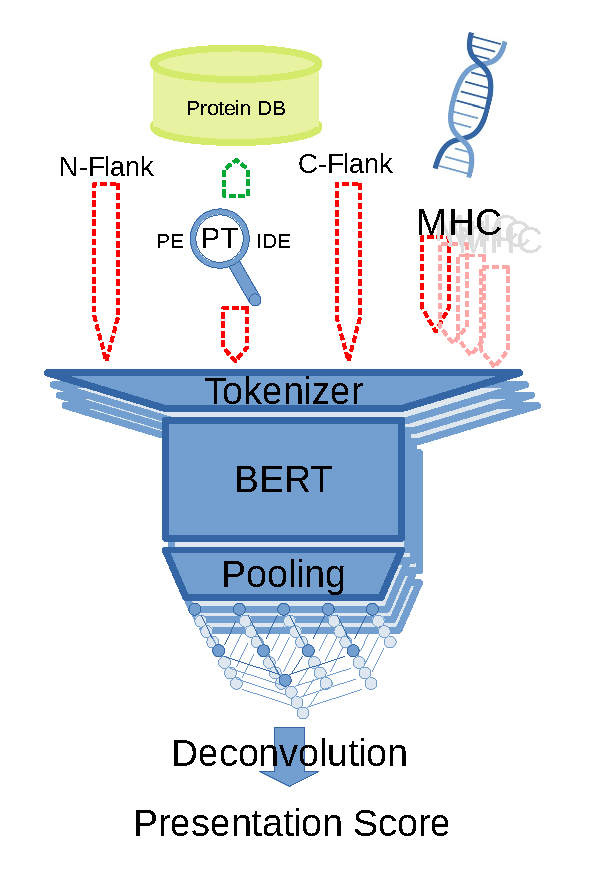
\includegraphics[width=0.38\textwidth]{summary.pdf}
		\caption{Graphical summary}	
	 	\label{fig:summary}
		}
	\end{wrapfigure}
	One of the biggest obstacles faced in prolonging human life expectancy in high income countries today is cancer. In addition, recent events have highlighted that viruses still pose a serious threat. The \gls{MHC} class-I pathway facilitates the detection of both of these by the immune system. It presents parts of proteins present inside a cell (peptides) on its membrane surface. If visiting immune cells detect non-self peptides, they can terminate the cell. 

Being able to predict which peptides will get presented and which not can help improve the efficiency of certain therapies. Current \gls{SOTA} models mainly use ensembles of shallow fully connected neural networks. In this thesis, we explore the application of \acrshort{BERT} to this task and use modern interpretation frameworks to gain biological insights.

	As can be seen in Figure \ref{fig:summary} our model (ImmunoBERT) takes as input an amino acid sequence consisting of several parts. The main one is the peptide for which we want to predict presentation. The next one is the peptide's surrounding in its source protein - which is the result of mapping the peptide to a protein database. And finally, we also input a representation of the \gls{MHC} class I protein which potentially presented the peptide. We use a novel representation for this sequence and feed it into a \acrshort{BERT} model. Based on experiments we chose a fitting pooling layer and feed its output into a multilayer perceptron. The fact that there are up to six \gls{MHC} proteins in each individual is a complication that requires us to perform deconvolution.

	Using motifs and a novel application of \acrshort{SHAP} and \acrshort{LIME}  to this domain, we identify the most important parts of the input sequence. In particular, we find that amino acids close to the N- and C-terminals of the peptides are highly important. Also, some positions of \gls{MHC} proteins (in particular in the A, B and F pockets) are often assigned a high importance ranking. We also observe that the flanks have little importance and this decreases with distance to the peptide.

}

\maketitle

\section*{Acknowledgements}
This thesis would not have been possible without the support and understanding my parents have provided throughout my life. Thank you for this - in particular for being so accepting of my extraordinary career choices.

It would also not have been possible without Ajitha Rajan, Javier Alfaro and Georges Bedran who have proposed this exciting area of research, were always happy to speak about the project and through discussions jointly supervised the project. Thank you.

Also, I thank the PL-Grid and CI-TASK Infrastructure, Poland, for providing their hardware and software resources.

\newpage\standarddeclaration



\tableofcontents

\end{preliminary}

\chapter{Introduction}
The immune system defends the human body from a broad range of threats. Some of these manifest inside the body's own cells. For example viruses and cancer both utilize the cell's gene expression system to facilitate their own reproduction and spreading. \gls{CTL}, a special kind of T-cells, can detect affected cells and terminate them. To do so, they require a way to `look inside' the body's cells. A system revolving around the \gls{MHC} proteins facilitates this in many higher vertebrates \cite{encyclopaedia_britannica_major_2021}. \gls{MHC} proteins are also called \gls{HLA} in humans. This thesis focuses on the \gls{MHC-I} proteins and their antigen presentation pathway which is active in all nucleated cells of the human body \cite{mosaad_clinical_2015}. Proteins present in these cells are constantly being fragmented into smaller pieces - so called peptides. These then bind to the \gls{MHC} proteins forming \glspl{pMHC}, which are then transported to the cell membrane. There, the peptides get presented on their `MHC pedestal' to the outside world. The  \gls{pMHC} are antigens for the \glspl{TCR}. The exact part of the antigen where the \gls{TCR} binds is also called an epitope. \cite{murphy_janeways_2017, gasser_informatics_2021} 

An infection by a virus or a cancer causing mutation, can both result in the production of proteins that would otherwise not be present in a healthy cell. Eventually this leads to the presentation of neo-antigens (non-self \gls{pMHC}) to the outside world \cite{schumacher_neoantigens_2015, zhang_neoantigen_2021}. Dependent on whether the \gls{CTL} consider the peptides presented to them as self or non-self, they decide to terminate the cell. The human body, therefore, already has the ability to fight viruses and cancers. Many cancers, however, have evolved mechanisms to circumvent the immune system. An example is tumor-induced immune suppression \cite{fehres_understanding_2014}. Check-point inhibitors are used to counter this. Peptide-based vaccines are another tool that can be used to strengthen the immune response. Identifying which peptides will most likely be presented by a cancerous cell and elicit an immune response (immunogenic peptides \cite{li_deepimmuno_2021}) is an important component in the development of peptide-based vaccines \cite{comber_mhc_2014}. One way to achieve this \textit{in silico}, is by utilizing \gls{ML}. The usage of the \acrshort{BERT} model to predict the first part of this - peptide presentation, is the topic of this thesis. 

Although an important step, presenting foreign peptides (neo-antigens) is not sufficient to elicit an immune response. For example, the presented peptide needs to bind sufficiently strong to a \gls{TCR} as well. This step is not part of our analysis. Another group of models deals with this step (for example DeepImmuno \cite{li_deepimmuno_2021}). Many other factors need to be considered as well in vaccine development. For example, the \gls{MHC-I} pathway is typically only capable of presenting the cell's endogenous protein fragments. Several methods can be used to internalize the peptides from a vaccine. For example professional antigen presenting cells (e.g. dendritic cells) can internalize exogenous material and then present it to the outside world via the \gls{MHC-I} pathway. Glycans and other adjuvants might be required to facilitate the vaccine uptake \cite{fehres_understanding_2014}. This is an active research area.

As stated above, this thesis explores the application of the \acrshort{BERT} architecture to the epitope presentation prediction via the \gls{MHC-I} pathway in humans. To do so we first develop a for this problem novel architecture based on a pretrained \acrshort{BERT} model. The resulting model achieves competitive performance to current \gls{SOTA} models on an independently curated benchmark set. In addition, a motif analysis confirms that our model has indeed learnt \gls{MHC} allele dependent peptide specificities. In a novel step we then apply \acrshort{SHAP} and \acrshort{LIME} to find the parts of the peptide, \gls{MHC} protein and surrounding flanks of the peptide, that are particularly relevant for presentation.

Chapter \ref{chapter:background} presents the relevant biological and \gls{ML} concepts before lining out the current \gls{SOTA} in T cell epitope prediction. Then Chapter \ref{chapter:method} introduces the datasets and methodology we used. The results achieved and the interpretation are presented in Chapter \ref{chapter:results}. We finish with a small discussion and suggestion for future research in Chapter \ref{chapter:conclusion}.


\chapter{Background}
\label{chapter:background}

	A solid understanding of the underlying biology is required to design a model capable of predicting the peptides presented by a cell. So, this is introduced before the relevant \gls{ML} concepts.

\section{Biology}
\label{sec:biology}
	Our discussion of the biology begins with a subsection about proteins, which also lines out why peptide presentation is a suitable mechanism to transfer information about a cell's state of health to the outside world. Then we present the \gls{MHC-I} pathway that implements the presentation process. The experimental datasources used for its examination in the context of presentation prediction are discussed then. Finally, we will introduce the \gls{MHC} protein and its naming convention.

	\subsection{Proteins}
	\label{subsec:bg_biology_proteins}

		Proteins play a central role in the human body. They consist of \glspl{AA} chained together via peptide bonds \cite{pollard_cell_2016}. In general, an \gls{AA} consists of an amino group a central carbon (with a hydrogen atom), an \gls{AA} specific side chain and on the opposite side to the amino group, there is a carboxyl group \cite{crowe_chemistry_2014}. During the formation of the peptide bond, the carboxyl group  of one \gls{AA} is connected to the amino group of the next one. The end of the chain with the amino group is called N-terminus the end with the carboxyl group is called C-terminus. There are 20 \glspl{AA} encoded by the genetic code \cite{pollard_cell_2016}. Each of them can be represented by a letter. Once joined together by peptide bonds, we refer to the single \glspl{AA} as residues. Short chains of residues are referred to as peptides, while longer ones are referred to as polypeptides.
		
		The blueprints for the proteins produced by a cell are stored in \gls{DNA} molecules. These are chains of nucleotides. Each nucleotide contains one of four bases. Parts of these very long \gls{DNA} molecules can be transcribed (copied) into shorter \gls{mRNA} molecules. Dependent on the bases, ribosomes then translate groups of three \gls{mRNA} nucleotides into \glspl{AA} that get appended to a protein in production \cite{pollard_cell_2016}.
	
		While peptides behave like flexible strings, longer polypeptide chains and proteins typically adopt a 3D molecule structure due to the features of their residues (e.g. hydrophobic and hydrophilic regions) and bonds forming between them. We distinguish four levels of protein structure - with the lower levels influencing the emergence of the higher ones \cite{crowe_chemistry_2014}. Primary structure refers to the polypeptide's sequence of \glspl{AA}. It can be represented as letters (one per \gls{AA}), written from N to C-terminus. Due to hydrogen bonds forming between distant \glspl{AA} in the polypeptide a secondary structure emerges. This could be structural features like $\alpha$-helices and $\beta$-sheets. These secondary structures can get packed to form regions of defined 3D shape - tertiary structures like $\beta$-barrels or coiled coils. Eventually, several of these (then called domains or subunits) can combine - referred to as quaternary structure \cite{crowe_chemistry_2014}.
	
		In eukaryotic proteins, one domain often corresponds to one exon (translated area of the gene code, interrupted by introns - not translated ones). Similar exons coding for similar domains are often found at distant parts of the genome. They are like "modules" that can be used in several proteins. The genes coding for these typically share a common ancestor. Such a relationship is referred to as homology and they are often similar on a functional level but may differ in \gls{AA} sequence \cite[Chapter 3]{pollard_cell_2016}. This makes splitting up the dataset into train, test and validation set to assess generalization capability more complex (see Subsection \ref{subsec:split}).
	
		Proteins perform tasks as diverse as breaking up nutrition into its components, muscle movement and sustaining cell structure. Because of the wide range of functions they can perform, controlling which proteins are present in a cell is so important. For example, cancer is essentially a set of \gls{DNA} mutations (and/or epigenetic changes) that change cell behaviour by causing changes to the cell's proteome. In healthy cells, cell division is  strictly controlled and most cells enter a non-dividing state. However, if sufficient pathogenic changes to the genetic material accumulate, the brakes on this system can loosen (e.g. due to mutations that render tumour suppressor proteins useless) and the inappropriate activation of oncogenes (supporting cell division) can lead to uncontrolled propagation of the tumour \cite[Chapter 41, Section X]{pollard_cell_2016}. In comparison, a defining feature of viruses is their inability to reproduce themselves. They, therefore, need to capture the host's protein expression system to do so. This will also lead to changes to the cell's proteome.

	\subsection{The MHC class-I pathway}
	\label{subsec:bg_biology_pathway}
		Therefore, presenting information about the proteins present inside the cell transfers valuable information about the cell's state of health to the outside world. This is achieved via the \gls{MHC-I} pathway which has the following steps \cite{rock_present_2016}:
	
		\begin{itemize}
			\item[1.] Proteasomes fragment the cell's internal proteins into peptides
			\item[2.] \gls{TAP} proteins transport these peptides into the \gls{ER}
			\item[3.] In the \gls{ER} there reside membrane bound \gls{MHC-I} proteins, which can bind with the peptides to form \gls{pMHC}.
			\item[4.] The \glspl{pMHC} get transported to the cell membrane, where the \gls{MHC} protein acts as a pedestal for the peptide and presents it to the extracellular fluid 
			\item[5.] A \gls{CTL} with a fitting \gls{TCR} could bind a presented neo-antigen. This might trigger an immune reaction, as \glspl{CTL} do not strongly bind to "self" peptides (the body's own peptides) but only non-self ones. \glspl{CTL} are trained for this in the thymus by positive- and negative selection \cite{murphy_janeways_2017}.
		\end{itemize}
	
		With regards to step 1 Figure \ref{MHCpathway} shows that inside the cell's cytoplasm, proteins are constantly degraded into peptides (mostly of 7-8 \glspl{AA} length \cite{nielsen_immunoinformatics_2020}) by proteasomes. There are three different types of proteasomes, having different specificities \cite{rock_present_2016}. While the proteasomes generate the exact C-terminal cut, the produced fragments can further be cut down by peptidases on their N-terminals in the cytoplasm \cite{nielsen_role_2005}. To reach the \gls{ER} these are bound by \gls{TAP} proteins that are responsible for the peptides' transfer to the \gls{ER} (step 2). The affinity of these \gls{TAP} proteins peaks at peptide lengths of 11 \gls{AA} \cite{nielsen_immunoinformatics_2020}. Since the peptides go through both filters - proteasomes and \gls{TAP} - the distribution of those making it to the \gls{ER} concentrates at 9-10 \glspl{AA}. With regards to sequence specificity, \gls{MHC} binding is far more restrictive than proteasomal cleavage as well as \gls{TAP} transport and it seems their main role is to deliver right length peptides to the \gls{ER} and not to act as a sequence filter \cite{nielsen_immunoinformatics_2020}.
	
		In the \gls{ER} the peptides encounter membrane bound \gls{MHC} proteins. It has been shown that the binding of \gls{MHC} proteins to peptides (step 3) is a particularly restrictive step in the \gls{MHC-I} pathway - with only roughly 1 in 200 randomly generated peptides binding \cite{yewdell_immunodominance_1999}. These \gls{MHC} proteins differ between individuals. In fact, each individual has several different \gls{MHC} proteins as well. Within the human MHC located on chromosome 6 at 6p21.3 there are three main loci coding for \gls{MHC-I} proteins: HLA-A, HLA-B and HLA-C \cite{mosaad_clinical_2015}. As \textit{Homo sapiens} is a diploid species, each human therefore can express up to six different HLA-A, HLA-B and HLA-C proteins. Each of those can have different binding properties. As these gene regions are highly polymorphic and there are many different \gls{HLA} alleles in the human population, there is a large variety in immunopeptidomes (the entirety of all presented peptides) across humanity. In fact, currently there are more than  4,064 HLA-A, 4,962 HLA-B and 3,831 HLA-C proteins known \cite{ebi_immuno_2021}. Each of these can bind roughly 1,000 to 10,000 different peptides \cite{abelin_mass_2017}.
	
		If the binding between \gls{MHC} and peptide in step 3 is successful, a complex (\gls{pMHC}) forms. This can then migrate to the cell membrane. Here, the peptide is presented to the extracellular environment by the \gls{MHC} protein - which acts as a pedestal for the peptide (step 4). Whether this results in an immune reaction or not, depends on whether a \gls{CTL} with a fitting \gls{TCR} gets in contact with the \gls{pMHC} and the presence or absence of other signals. Approximately half of the peptides will not be detected due to a limited \gls{TCR} (CD8+) repertoire \cite{yewdell_immunodominance_1999}. In total, \cite{yewdell_immunodominance_1999} estimate that just one out of 2000 random peptides (8-11 \gls{AA} long) of a foreign antigen will be presented by a particular \gls{MHC} protein and cause an immune reaction. 
		
		Interestingly, in addition to their role in adaptive immunity, \gls{MHC} proteins also have an inhibitory influence on natural killer cells \cite{mosaad_clinical_2015} (part of innate immunity). This way, a tumour cell that switches off \gls{MHC} production completely will also be destroyed. However, what happens after peptide presentation at the cell surface is not part of our examination.
	
		\begin{figure}
			\centering
			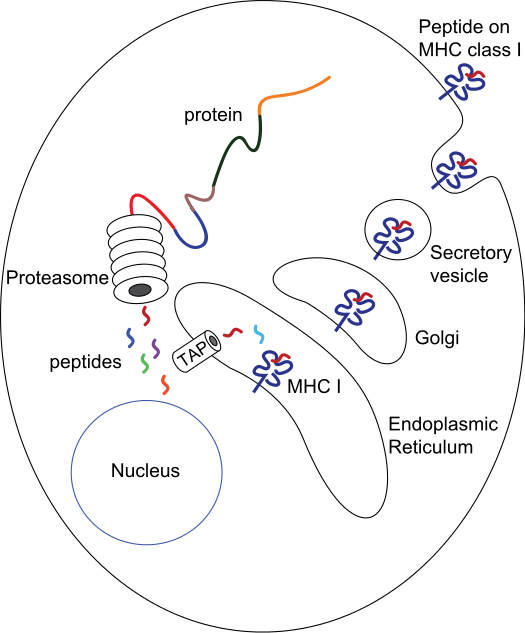
\includegraphics[width=60mm]{525px-MHC_Class_I_processing.svg.png}
			\caption[MHCpathway]{\gls{MHC-I} pathway \cite{wikipedia_major_2021}}
			\label{MHCpathway}
		\end{figure}

	\subsection{Experimental datasources}
		As the most restrictive step in epitope presentation is \gls{MHC} binding, measuring the \gls{BA} between a particular \gls{MHC} protein and a peptide \textit{in vitro}, can give us some insight into how likely it is that a particular peptide will be presented to the extracellular environment. Early presentation predictors were, therefore, only trained on this \gls{BA} data. Its biggest disadvantage is, that it is costly to carry out the experiments that then only generate little data \cite{alvarez_nnalign_ma_2019}.

		In the modern high throughput \gls{EL} approach, the whole immunopeptidome of the cell is harvested and then the peptides are identified using mass spectrometry \cite{hunt_characterization_1992}. This identifies many peptides at once. However, it is typically not possible to measure which of the up to six different \gls{MHC} alleles presented which eluted peptide. Monoclonal cell lines, that only express a single \gls{MHC} allele are a potential way around this limitation. There also exist algorithms to identify which allele is responsible for a peptide's presentation. This step is called ``deconvolution'' in the literature. However, it  also often relies on data that can be unambiguously ascribed to a single allele to  kickstart it (see Subsection \ref{subsec:deconv}).

		Another disadvantage of the \gls{EL} approach is, that it does not generate definitive negative examples. It only reports about the presence of a peptide at the cell's surface. It cannot assert the absence of a peptide from the individuals immunopeptidome. For example a peptide present in the human genome, might only not be presented by the cell because its protein is not being expressed by the particular cell. Despite it's drawbacks, the high quantity of data generated by this approach will make it the backbone of our examinations.
	
	\subsection{MHC proteins and peptide binding}
	\label{subsec:bg_biology_mhc}
		There are several types of \gls{MHC} proteins. We will only concentrate on the classical \gls{MHC-I} proteins here. Each of those is a hetero-dimer consisting of the non-covalently bound transmembrane heavy chain $\alpha$ and the light chain $\beta_2$-microglobulin \cite{stryhn_longer_2000}. The $\alpha$ chain has two membrane distal $\alpha_1$ and $\alpha_2$ domains that form a potentially peptide binding groove. The $\alpha_1$ and $\alpha_2$ domains each consist of a sheet of four antiparallel beta strands and a single helical region. The beta sheets of the two $\alpha$ domains together, form the floor of the groove, while the helices each form one of its sides \cite{lefranc_imgt_2005}. The residues lining this groove are also the ones showing the highest number of polymorphism. Six pockets (A-F) were identified for peptide binding. In particular pockets A and F are responsible for binding the peptide's N- and C-termini \cite{stryhn_longer_2000}. Most peptides are firmly embedded into the binding groove and terminated on both sites by the A and F pocket. So, there is little variation with regards to bound peptide length. Bulges and in a very few cases protrusions out of the groove can, however, lead to longer peptides binding \cite{stryhn_longer_2000}.
	
		As already mentioned, there are many different MHC alleles. So, the following naming convention has been adopted in humans \cite{hla_informatics_group_hla_nodate}. The full name of a MHC allele could look like: HLA-A*04:18:03:01N. The letter after \gls{HLA} ('A') signifies the gene that we are referring to. Then, the following number ('04') stands for the allele group. This often corresponds to the serological antigen carried by it. The second number ('18') refers to the subtype. Importantly, \gls{HLA} alleles that differ in any of those three parts ('A', '04' or '18'), will also differ on an amino acid level. So, these parts determine the specific \gls{HLA} protein. In contrast, the third number ('03') only signifies substitution mutations in the gene that do not lead to a different protein. The last number ('01') orders the alleles with respect to mutations in the introns. Finally, the suffix ('N') can be used to transfer information about the expression of the allele. For example, if an allele would not be present on the cell surface. For our purposes, we will only consider the gene and the first two numbers.
			
		Differences in \gls{HLA} proteins present in an individual do have real world consequences. For example, while HLA-B*42:01 is linked to better outcomes for HIV sufferers, HLA-B*42:02 is not, despite them only differing in one amino acid position \cite{van_deutekom_zooming_2015}. In contrast, HLA-B*35:03 is suspected to be connected with fast AIDS progression, while the only at one position differing allele HLA-B*35:01 is not \cite{van_deutekom_zooming_2015}. The differences are not limited to viral infections. In the Gambia HLA-B*53 was shown to be present in 25\% of healthy and mild malaria cases while only to be present in 15\% of severe cases - suggesting an approximately 40\% reduction in the risk of severe malaria \cite{mosaad_clinical_2015}.

\section{Machine Learning}
	Based on the last section, predicting the immunopeptidome of a particular individual is difficult mainly because of three facts. First, as any of the up to six \gls{MHC-I} alleles present in the cell might be responsible for a peptide observation in an \gls{EL} experiment, the problem does not fit well into the supervised learning framework in which x results in y. Second, the high throughput eluted ligand assays only produce positive examples resulting in the need to create artificial negative ones (decoys). This is, third, aggravated by the fact that in reality most peptides will not be presented on the cell's surface (imbalanced dataset). In this section we discuss these issues in turn and then present the backbone architecture used by us  - \acrshort{BERT}, before introducing the techniques we will employ for its interpretation.
	
	\subsection{Deconvolution}
	\label{subsec:deconv}
		With regards to the first obstacle, deconvolution refers to the process in which each peptide is associated to its presenting \gls{MHC} protein \cite{alvarez_nnalign_ma_2019}. Several approaches have been put forward to deal with this challenging task. We already mentioned the possibility to use cell lines only expressing a single \gls{MHC} allele. However, bioinformatics has also produced \textit{in silico} ways to tackle this task. For example the usage of unsupervised sequence clustering - like Gibbs clustering. This, however, needs manual curation like providing the correct number of clusters and sometimes also during the assignment of those clusters to \gls{MHC} proteins \cite{alvarez_nnalign_ma_2019}. As an alternative, \cite{bassani-sternberg_unsupervised_2016} have developed a mixture model approach that models the likelihood of the observed eluted ligands of a sample (with up to six different \gls{HLA} proteins) as the mixture of several \glspl{PWM}. They observe that most of the observed peptides show a good match to only one of those \glspl{PWM} and so can be assigned to this. These \glspl{PWM} are then assigned to known \glspl{PWM} of alleles from IEDB. 

		Looking at deconvolution from the perspective of weakly supervised learning - in particular \gls{MIL} - points us towards solutions based on single allele models. \gls{MIL} assumes that several instances $x_{n_j}$ do each belong to a class $y_{n_j} = 1$ or not $y_{n_j} = 0$. However, these $y_{n_j}$ are not directly observed. We only know the classifications $y_n$ for bags $X_n$ of instances ($X_n = (x_{n_1}, x_{n_2}, ..., x_{n_m})$). The presence of a single instance belonging to a class in a bag is sufficient for the whole bag to be labelled with this class ( $\exists j, y_{n_j} = 1 \Rightarrow y_n = 1$). Only if all instances do not belong to the class, then the bag's label is zero ($\forall j, y_{n_j} = 0 \Rightarrow y_n = 0$). This means that $y_n = \textrm{max}_j y_{n_j}$ \cite{ilse_attention-based_2018}. These bag level labels $y_n$ are what is contained in the data. There are two main categories of \gls{MIL} algorithms \cite{wang_revisiting_2018, ilse_attention-based_2018}. The traditional approach is instance-level based while the alternative is embedding-level based. 
		
		In instance-level based methods, a function $f$ estimates the classification for each instance $\hat{y_{n_j}} = f(x_{n_j})$. The class of the whole bag is estimated as the maximum estimate of the bag's instances $\hat{y_n} = F(X_n)=\textrm{max}_j f(x_{n_j})$ \cite{ramon_multi_2000}. In contrast, in embedding-level approaches, $f$ does not directly estimate the instance's classification but only produces an embedding. A pooling operation is used to obtain a fixed dimensional representation of the whole bag. This representation is then fed into a classifier for the whole bag. Although \cite{wang_revisiting_2018} have demonstrated, that the  latter approach can have higher performance, we will stick to the former one as it fits better to the fact, that our data also contains observations that can be clearly assigned to a single allele. Also, the traditional approach is implicitly loosely followed by NetMHCpan's deconvolution mechanism \cite{alvarez_nnalign_ma_2019} and BERTMHC \cite{cheng_bertmhc_2020}.

		So, in the instance-level approach the estimation for the bag's classification is the maximum of the individual estimates. The maximum is not differentiable everywhere which is a requirement for gradient based learning algorithms. There is, however, a differentiable version of the $max$ available - the LogSumExp ($\max_j x_j \approx \frac{1}{\beta}\log \sum \exp \beta x_j$). However, since the astonishing success of the ReLU activation function in neural networks, the concerns about not being differentiable locally seem to have eased a bit and we will see that the current \gls{SOTA} model NetMHCpan also implicitly relies on the $\max$ pooling via the NNAlign\_MA framework (see Subsection \ref{subsec:netmhcpan}).



	\subsection{Negative examples}
	\label{subsec:negative}
		The previous section argued that our problem differs from the traditional supervised learning setting with regards to the inputs. Here we argue, that it also differs with regards to the output. In the supervised setting, the training data is assumed to be fully labelled \cite{bekker_learning_2020}. However, in our case, there are no (few if we were to include \gls{BA} data) negative examples available. We do have a lot of positive examples (peptides eluted from the cell's surface) and even more unlabelled data (the whole part of the human proteome expressed in a sample). This fits into the category of \gls{PU} learning, which is closely linked to the problem of one-class classification in which only positive examples are available. \cite{elkan_learning_2008} have analysed the \gls{PU} setting in particular with regards to the transporter classification database for membrane transport protein analyses (TCDB) which stores proteins involved in signalling across membranes (positive examples) and the SwissProt database (unlabelled examples). In addition to the input variable $x$ and the class label $y \in \{0, 1\}$ they introduce $s$, that signifies whether an example is labeled ($s = 1$) or not ($s = 0$) and assume:
		
		\begin{itemize}
			\item Only positive examples are labeled: $P(s=1 | x, y=0) = 0$
			\item For a positive example, whether it is labelled or not is independent of $x$: \\ $c = P(s  = 1 | x, y=1) = P(s = 1 | y = 1)$
		\end{itemize}
	
		They call a classifier $g(x) = P(s = 1 | x)$ that distinguishes between labelled and unlabelled examples a non-traditional classifier and proof that:
		\begin{equation}
			P(y = 1 | x) = \frac{P(s = 1 | x)}{c}
			\label{equ:PU}
		\end{equation}
		
		Therefore, $f(x) = \frac{g(x)}{c}$ is a traditional classifier for the original class. Furthermore, \cite{elkan_learning_2008} show three ways to estimate $c$ using the non-traditional classifier $g$ and a validation set $V$, consisting of positive ($P$) and unlabelled data. The first estimator is $\hat c_1 = \frac{1}{|P|}\sum_{x \in P}  g(x)$, the second $\hat c_2 = \frac{\sum_{x \in P} g(x)}{\sum_{x \in V}g(x)}$ and the third one $\hat c_3 = \textrm{max}_{x \in V}g(x)$. These estimators rely on the classifier $g$ being powerful enough to capture the probability exactly (not mis-specified). They argue, that if $g(x) = P(s = 1 | x)$ only approximately, then $\hat c_1$ is the best choice.
		
		While Equation \ref{equ:PU} directly points towards adjusting the threshold of $g(x)$, that is typically 0.5 to the value $\frac{0.5}{\hat c_1}$ to construct the classifier $f(x)$ for the actual class we are interested in predicting, they also propose a second way that leaves the threshold unchanged to achieve this. This relies on splitting up every unlabelled example into a positive one and a negative one and train the classifier using different weights for these. In an example analysis they perform with the TCDB and SwissProt data mentioned before, they find that those two versions perform similarly well.
		
		Their results deliver the theoretical justification for our approach. However, we will not re-scale the threshold since we will only benchmark our classifier vs generated negative data (decoys). If we, however, were to use it for real prediction, we would have to scale the threshold in accordance to Equation \ref{equ:PU}.		

	\subsection{Imbalanced datasets and metrics}
	\label{subsec:imbalanced}
		Although we only have positive examples, the unobserved implicit negative ones outweigh the observed positive ones by a considerable margin as only one out of roughly 200 randomly generated peptides will bind (see Subsection \ref{subsec:bg_biology_pathway}). This raises the question of how to deal with this imbalance. Many standard learning algorithms experience significant problems when dealing with imbalanced data - however to what degree the original dataset should be balanced is still open to debate \cite{he_learning_2009}. It seems that it has to be answered on a case by case basis. However, \citeauthor{weiss_learning_2003} \cite{weiss_learning_2003} have shown that selecting accuracy as the relevant performance metric tends to favour sticking close to the natural class distribution, while selecting \gls{AUC} based metrics favours more balanced class distributions.
		
		\citeauthor{he_learning_2009} \cite{he_learning_2009} argue, that accuracy is in general not a good metric when assessing performance on highly skewed datasets. If the majority- to minority class ratio was 999:1, then a classifier always predicting the majority class has an accuracy of 99.9\% - despite it missing all minority class examples. There are alternative metrics available that result in a more balanced assessment.
		
		A typical binary classifier scores an example with values between 0 and 1. Scores above a predefined threshold are considered positive (belonging to the class), those below negative. If a positive prediction is correct, it is a \gls{TP} example, if incorrect a \gls{FP} one. Equally, a correct negative assignment is a \gls{TN} example, and an incorrect one a \gls{FN}. In the equations below, TP(threshold) means the threshold dependent count of all \gls{TP} examples across the relevant dataset. Equivalently, \gls{FP}, \gls{TN} and \gls{FN} are defined \cite{he_learning_2009}:
		\begin{align}
		    \textrm{Recall or TPR(threshold)} &= \frac{TP(threshold)}{TP(threshold) + FN(threshold)} \label{eq:RECALL_TPR} \\
		    \textrm{FPR(threshold)} &= \frac{FP(threshold)}{FP(threshold) + TN(threshold)} \label{eq:FPR} \\
		    \textrm{Precision(threshold)} &= \frac{TP(threshold)}{TP(threshold) + FP(threshold)} \label{eq:PRECISION} \\
		    \textrm{AP} &= \sum_n (Recall(T_n) - Recall(T_{n-1})) \cdot Precision(T_n) \label{eq:AP} 
		\end{align}
		
		A common way to visualize a classifier's diagnostic ability is the \gls{ROC}. It emerges when we let the classifier's threshold slowly increase from zero to one and plot the \gls{FPR} (Equation \ref{eq:FPR}) on the x-axis and the \gls{TPR} (Equation \ref{eq:RECALL_TPR}) on the y-axis. A good classifier will have a high area under this emerging curve - the \gls{AUC}-\gls{ROC}.
		
		An alternative visualizations are \gls{PR} curves. They emerge, when we let the threshold slowly increase from zero to one and plot the recall (Equation \ref{eq:RECALL_TPR}) on the x-axis and the precision (Equation \ref{eq:PRECISION}) on the y-axis. The \gls{AP} \cite{sklearn_sklearnmetricsaverage_precision_score_2021} is a common way to summarize a \gls{PR} curve. It is calculated based on a series of increasing threshold values ($T_n$, see Equation \ref{eq:AP}). 
		
		We will use the \gls{AUC}-\gls{ROC} due to its easy interpretation. However, \cite{he_learning_2009} argue that \gls{PR} curves provide a more informative representation of a model's performance under highly imbalanced data. Therefore, we will visualize the performance using \gls{PR} curves and also calculate the \gls{AP} metric.

	\subsection{BERT}
	\label{subsec:BERT}
		The backbone of our classifier is a \gls{BERT} \cite{devlin_bert_2019} model. This belongs to the Transformer class of neural networks that have been pushing the \gls{SOTA} performance in many natural language processing tasks. In particular big models like GPT-3 \cite{brown_language_2020} have captured the public's imagination \cite{weinberg_philosophers_2020}. While the original Transformer consists of an encoder and a decoder \cite{vaswani_attention_2017}, \gls{BERT} only has an encoder stack, producing one contextualized embedding for each input token.

		The revolutionary idea in transformers is the consequent usage of self-attention layers - signified by the original paper's title "All you need is attention" \cite{vaswani_attention_2017}. Attention enables a neuron to focus on the output of any preceding layer position. Crucially, it can focus on far away positions and directly access their outputs - without them going through many operations. This is particularly useful when dealing with long sequence data. In comparison, recursive neural networks struggle to take into account far away text parts (long-range dependencies) and are prone to vanishing gradients \cite{vaswani_attention_2017, yannic_kilcher_attention_2017,  dosovitskiy_image_2020}. More recently, these advantageous properties of transformers have also been exploited for visual tasks by \cite{dosovitskiy_image_2020}. While \glspl{CNN} can connect information from two distinct points in a picture only in their upper layers (small receptive fields in low ones), transformers can do this already in early ones \cite{dosovitskiy_image_2020}.
		
		Transformers use a very special type of attention. There are in general three types of attention. Hard attention, soft attention and self-attention \cite{antoniou_mlp_2020}. Let us assume that for each example, a lower layer produces $n$ vectors $o_j$ as output. In our setting, each of these $n$ vectors could correspond to an amino acid of a peptide we want to classify.	
		Hard attention would only consider a subset of $m \leq n$ of these as input for the next higher layer - completely disregarding the others. This is a non-differentiable operation that we will not consider any further in this thesis. 
		Soft-attention, in comparison, is often used for pooling. It calculates weights for each $o_j$ (e.g. by calculating the dot product of a learned vector with all $o_j$ followed by a softmax operation). The weighted sum of the $o_j$ is then the single fixed dimensional input vector to the following layer \cite{toshniwal_cross-task_2020}. We will come back  to this again when we discuss the various ways of pooling the output of our model's \gls{BERT} backbone before feeding it into the classifier's head. 
		Finally, self-attention is the form of attention used by transformers \cite{vaswani_attention_2017}. The standard implementation uses learned transformations to produce a value $v_j$, query $q_j$ and key $k_j$ vector for each output vector $o_j$. An intuitive way to think about those is to see the key vector as encoding what type of information is encoded in the position (similarly to the key in e.g. a hash table). The query vector then encodes which type of information a position in the next layer requires as input. If the information encoded at position $j$ and the information required at position $i$ are similar, then $k_i$ and $q_k$ should be similar. Therefore, a dot product (cosine simularity) is calculated for each of the $n^2$ possible position pairs. This represents the weighting that the $v_j$ will have in the input to position $i$. In addition, \gls{BERT} performs several of these in parallel (multiple heads), allowing a neuron to focus on several aspects at once.
		
		Although transformers have been successful in tackling the long-range dependency issue, their biggest strength is also their biggest weakness. Self-attention assesses the importance of each lower layer output for each higher layer input. This defines a squared complexity task \cite{lukasz_kaiser_attention_2017}. Therefore, \gls{BERT} models are often limited to relatively short sequence lengths. There are initiatives to alleviate this. For example google's Reformer \cite{kitaev_reformer_2020} network uses the sparseness of the attention matrix. Using locality sensitive hashing allows them to focus the attention calculation on the values with the closest indices to the keys. This approach allows them to reduce the complexity of the self-attention operation to $n\log(n)$. The application of these optimized models to our task is an promising area for future research.
		
		\textbf{BERT pretraining: } The \gls{BERT} framework \cite{devlin_bert_2019} postulates two steps in training a model for a new task - pretraining and fine-tuning. For pretraining, a vast amount of unlabelled data is used to perform self-supervised learning tasks. The original \gls{BERT} paper \cite{devlin_bert_2019} uses \gls{MLM} and \gls{NSP}. In \gls{MLM}, part of an input sentence (typically 15\% of the tokens) are hidden - 80\% with a masking token, 10\% with a random token and 10\% with the same token. The model has to fill only those positions with their original tokens. This contrasts to de-noising auto-encoders, that reconstruct the whole original input \cite{devlin_bert_2019}. As \gls{MLM} allows and requires the network to use information from both sides of the gaps, it encourages the emergence of bidirectional representations for the input tokens. So, the final \gls{BERT} layer's outputs can be seen as \textit{context-sensitive} features. This contrasts to traditional embeddings, that are only dependent on a single token and not its context. By not always replacing the hidden parts with the masking token, \cite{devlin_bert_2019} want to alleviate the mismatch between pre-training vocabulary and fine-tuning vocabulary (which typically does not include the masking token). They also mention that keeping the transformer in the dark about exactly which parts have been replaced, forces it to keep a contextual representation of every position. To encapsule relationships between sentences, \gls{NSP} pretraining is used. This should prepare \gls{BERT} for tasks like question answering and natural language inference \cite{devlin_bert_2019}. The self-supervised learning task is to predict whether the second sentence input into the model follows after the first one. The pretrained protein \gls{BERT} model we use (\acrshort{TAPE}), was only pretrained using \gls{MLM}.

		\textbf{TAPE \cite{rao_evaluating_2019}: } In the domain of protein prediction, the \gls{TAPE} transformer model \cite{rao_evaluating_2019} implements the hugging face interface for the \gls{BERT} model. It has 12 layers with 12 attention heads each. It has been pretrained for 1 week on 4 GPUs on more than 32 million protein domains \cite[supplement]{rao_evaluating_2019} from the Pfam database using masked-token prediction (\gls{MLM}) \cite{pfam_tape_2019}. Next to the \gls{BERT} transformer model, \cite{rao_evaluating_2019} also pretrained several other models (\acrshort{LSTM}, \acrshort{ResNet}). 
	
		After the pretraining, they fine-tuned common \gls{SOTA} task specific model architectures using the embeddings generated from these models as well as baseline embeddings (like one hot encoded amino acids). During fine tuning they trained the full stack (including the pretrained model). The \gls{TAPE} framework includes tasks coming from three important areas of protein biology: structure prediction, detection of remote homologs and protein engineering. They find, that pretraining positively influences the performance on downstream tasks and that the best performing architecture (\gls{BERT}, \acrshort{LSTM}, \acrshort{ResNet}) for embedding generation is task dependent \cite[Table 2]{rao_evaluating_2019}. There are alternative protein transformer models available as well - like ProtTrans \cite{elnaggar_prottrans_2021}. However, due to its small size, our limited computing resources and that it has already been fine tuned previously for \gls{MHC-II} prediction (see Subsection \ref{subsec:BERTMHC}), we use the \gls{TAPE} transformer model as the backbone for our model.

		As transformers have shown impressive performance in many \gls{ML} tasks \cite{vaswani_attention_2017, brown_language_2020, dosovitskiy_image_2020, rao_evaluating_2019, elnaggar_prottrans_2021}, we want to explore whether they can also be applied to our task outlined in the introduction. Before, we present two frameworks for model interpretation and introduce the current \gls{SOTA} approaches in this field.
		
	\subsection{Interpretable AI}
	\label{subsec:interpretable_ai}
	To check, whether our model \textit{f} has learnt relationships grounded in biology, we employ two explanatory frameworks: \gls{LIME} \cite{ribeiro_why_2016} and \gls{SHAP} \cite{lundberg_unified_2017}.  We can only give a brief introduction on those two methods here.
	
	\textbf{LIME \cite{ribeiro_why_2016}:} As its name suggests, \gls{LIME} produces local (for a particular example) explanations, treating the model \textit{f} to be explained as a black-box (model-agnostic). It is motivated by the observation that simple models are often easy to explain but deliver worse performance than more complicated ones \cite{ribeiro_why_2016}. Therefore, the \gls{LIME} framework builds a surrogate model $g$ for the actual model's behaviour around a particular example $x$. The standard surrogate model used by the package is a ridge regression. This is trained to explain the original model's predictions. As input it receives interpretable data. This could be a binary vector $z'$ with the same dimension as the feature space of the original model. The binary vector is used to  generate a mutated example. Where a feature of the binary vector is 1, the feature value of the original example is used. Where the binary vector's feature is 0, an imputed value is used. The imputation is domain specific. We will use the text version. In this case, the feature $j$ (word) is just deleted if $z_j' = 0$. In contrast, \gls{LIME} tabular samples values from a Gaussian around the feature mean or the original feature - the \gls{LIME} package (https://github.com/marcotcr/lime) offers a lot of optionality here. The conversion from binary into original feature space is performed by the function $z = h_x(z')$ which depends on the example to explain $x$. In a next step, a distance to the original example is calculated, which is used as a weight for the sample in the training of the surrogate model. If a feature is particularly important for the prediction of the original example, then its addition in the binary feature should change the surrogate's estimate a lot. This means having a high coefficient.
	
	\textbf{Shapley values:} Although intuitively clear, \gls{LIME} has little theoretical grounding. In fact, it is well suitable to explain, how the predictions of the original model will change in the vicinity of the example to be explained, however, in general it fails to attribute the difference between the average prediction over the dataset and the example's prediction fairly to the various features. This is, because the only method that does this (and satisfies certain conditions) are Shapley values \cite{shapley_value_1953}, which measure the contribution of each feature value to the prediction for a particular example. Shapley values have their origin in game theory and are the only way to fairly attribute the outcome of a `game' satisfying four quite basic axioms \cite[supplement]{lundberg_unified_2017}:
	
	\begin{itemize}
		\item \textbf{Efficiency:} The sum of the Shapley values is equal to the original prediction
		\item \textbf{Symmetry:} If the inclusion of two features individually has the same effect on the estimator, then their Shapley values must be the same
		\item \textbf{Null effects:} Features not considered by the model, have a Shapley value of zero
		\item \textbf{Linearity:} A feature's, Shapley value for the sum of two models is the same as the sum of its Shapley values in the two models
	\end{itemize}
	
	A feature's Shapley value is computed by calculating the difference between the predicted value of a model trained to take into account that feature and one not taking it into account. This is done and averaged over all possible combinations of feature subsets, resulting in the feature's Shapley value. Equation \ref{equ:shapley} shows how the Shapley value of feature $i$ from the feature set $F$ is calculated for the prediction of an example $x$. $f_S$ denotes the model trained only on the features in set $S$ and $x_S$ the subset of $S$ features from $x$. Computing the whole expression is impractical for more than only a few features, due to the need to train and evaluate many models ($O(2^{\textrm{nr of features}})$). This led to the introduction of Shapley sampling values. These only sample a subset of all possible feature combinations and do not retrain models, but rather approximate the  impact of removing variables by marginalizing these over the training set \cite{lundberg_unified_2017}.
	\begin{align} 
		\phi_{i} 	& = \sum_{S \subseteq F \symbol{92} \{i\} }  \frac{|S|!(|F| - |S| - 1)!}{|F|!} [f_{S \cup \{i\}}(x_{S \cup \{i\} }) - f_{S}(x_S)] \quad 		&  \textrm{\cite[equation 4]{lundberg_unified_2017}} \label{equ:shapley} % \\
		% \phi_{i}(f, x) & = \sum_{z' \subseteq x'} \frac{(|z'| - 1)! (M - |z'|)!}{M!} [f_x(z') - f_x(z' \symbol{92} i)] \qquad 									& \cite[Errata]{lundberg_unified_2017} \label{equ:SHAP} 
	\end{align}
	
	\textbf{SHAP \cite{lundberg_unified_2017}:} Based on the idea of Shapley values, \citeauthor{lundberg_unified_2017} \cite{lundberg_unified_2017} developed the \gls{SHAP} package for the efficient approximation of \gls{SHAP} values. These are the Shapley values under the assumption that the model's output restricted to a subset of the features is given by the expected model prediction conditioned on this subset. 

	To estimate \gls{SHAP} values, the package offers several model specific ways as well as the model agnostic Kernel \gls{SHAP} which we will use. It is based on the observation that a linear explanation model (like \gls{LIME}) can be trained with certain parameters (in particular a special kernel) to approximate \gls{SHAP} values. However, while \gls{LIME} parameter choices are heuristic \cite{lundberg_unified_2017}, Kernel \gls{SHAP} trains the linear model in a specific way.
	Similarly to Shapley sampling values, Kernel \gls{SHAP} does not consider all possible feature combinations, but just a few. The standard value is 2048 + 2 times the number of features. In addition, to estimate the conditional expectations, Kernel \gls{SHAP} requires the data's background distribution. This is provided in the form of representative examples. Ideally, these are the whole training set. In total, if we had 20 features and a training set of 1000 examples, this would lead to 2.088.000 (=1000 x (2048 + 2x20) ) model predictions to estimate the \gls{SHAP} values. Therefore, the \gls{SHAP} developers suggest to use just few or only a single reference value for larger problems. The \gls{SHAP} values will then, however, only explain the difference in prediction vs this reference value and not the overall set.
	
	The main advantage of using a linear regression approximation vs directly the Shapley equations (see Equation \ref{equ:shapley}) is that the regressor can approximate all Shapley values at the same time - resulting in higher sample efficiency \cite{lundberg_unified_2017}.

\section{Current state of the art}
Now that we have discussed the necessary biological and machine learning methods, we want to take a look at the most popular models currently available. These have in particular evolved along three dimensions over the past decades. 

The first one regards their input data. As outlined in Subsection \ref{subsec:bg_biology_pathway}, the most restrictive step in the \gls{MHC-I} pathway is the binding of the \gls{MHC-I} protein with the peptide. Early models like \cite{nielsen_reliable_2003}, and in fact even quite recent ones like NetMHCpan-3.0 \cite{nielsen_netmhcpan-30_2016} were, therefore, just considering \gls{BA} data. Predicting binding affinity is theoretically a regression task. However, for example \cite{nielsen_netmhcpan-30_2016} transformed the binding affinity values to be between 0 and 1 by using the cut off transformation 1 - log(binding affinity IC50 in nM)/log(50,000). Also, an IC50 of 500 nM is often used as a threshold to distinguish between binders and non-binders \cite{paul_hla_2013, udaka_empirical_2002, reynisson_netmhcpan-41_2020, odonnell_mhcflurry_2020}. Newer models like NetMHCpan-4.1 \cite{reynisson_netmhcpan-41_2020} do typically also take into consideration \gls{EL} data. This data naturally defines a categorization task (presented, not presented). 

The second dimension of evolution, concerns the treatment of different MHC alleles. Early models were \gls{MHC} protein specific. This means that a single model is trained for a particular \gls{MHC} allele. Recent models typically also consider information about the \gls{MHC} protein concerned. This is often input via a pseudo sequence (subsequence of the \gls{MHC} protein's full amino acid sequence). Models able to deal with various \gls{MHC} alleles are often referred to as `pan' in the literature (e.g. NetMHC vs NetMHCpan). The next evolution step in this direction was the addition of deconvolution capabilities (see Subsection \ref{subsec:deconv}). 

Finally, the third dimension regards the context of the peptide. Most models still today do not take into account the amino acids surrounding the peptide in its source protein. However, based on the idea to capture the whole \gls{MHC-I} pathway, which also includes cleavage by proteasomes and proteases that might work better on certain contexts, models like MHCflurry \cite{odonnell_mhcflurry_2020} do exactly this. 

After this sketch of the evolution of \gls{MHC-I} immunopeptidome predicting models, we describe two of the most popular ones in more detail. Then we introduce one transformer model - BERTMHC - that has been trained for the prediction of peptide presentation by a related \gls{MHC} protein - the \gls{MHC-II} protein. This has been an important inspiration for our work. At the end of the section we give a very brief overview of some other notable approaches taken in the literature for binding affinity and/or presentation prediction.

	\subsection{NetMHCpan}
	\label{subsec:netmhcpan}
	
	The probably most commonly used model today is NetMHCpan. It has got a very long history which we could trace back to the early 2000s \cite{nielsen_reliable_2003} and is currently in its version 4.1 \cite{reynisson_netmhcpan-41_2020}. The 'pan' in its name means that it can handle various different \gls{MHC} proteins. NetMHCpan 4.1 is an ensemble of 50 single hidden layer feed forward neural networks. To support \gls{BA} as well as \gls{EL} data, the outputs of these networks have two heads \cite[supplement]{reynisson_netmhcpan-41_2020}. The information about the \gls{MHC} allele is given to the model in form of a pseudo sequence consisting of only 34 \glspl{AA}. These were identified by \cite{nielsen_netmhcpan_2007} as being particularly close to the presented peptide (closer than 4.0 angstrom from the peptide for a representative set of HLA-A and HLA-B structures). The idea is that those should be particularly relevant for peptide binding.

	For deconvolution of \gls{MA} data, NetMHCpan takes advantage of the NNAlign\_MA \cite{alvarez_nnalign_ma_2019} framework. First only \gls{SA} data is used to train a classifier (which takes as input a peptide and a single \gls{MHC} allele). Then follows the deconvolution step. Each observation that could be caused by multiple \gls{MHC} alleles, is deconvolved separately. To do so, the classifier trained in the previous step is used to predict the likelihood of each potential peptide:MHC protein combination independently. The \gls{MHC} allele showing the highest scaled prediction (the scaling essentially results in the z-score of allele's predictions) is chosen and used as the MHC protein responsible for the observation for all purposes until to the next deconvolution step. In case of a negative example, a \gls{MHC} allele is picked at random. Except for the scaling, this is also roughly the approach  we will follow. 
	
	The generation of negative examples is not explained in detail. However, \cite{alvarez_nnalign_ma_2019} say that they use random peptides from the UniProt database. For each peptide length they generate an equal amount of random negatives. This amount is five times the number of observations for the most abundant peptide length in a dataset (they combine several sources) \cite{alvarez_nnalign_ma_2019}. In total, it seems that for NetMHCpan there are roughly 18 negative examples per positive one in their training set  \cite[Supplement Table 1]{reynisson_netmhcpan-41_2020}.
	
	\subsection{MHCflurry}
	\label{subsec:mhcflurry}
	Next we introduce MHCflurry 2.0 \cite{odonnell_mhcflurry_2020}. It explicitly models the process of \gls{MHC} binding separately from the others (e.g. proteasomal cleavage). This results in a natural integration of \gls{BA} and \gls{EL} data. MHCflurry 2.0 consists of three sub-models. First, MHCflurry BA models the process of the peptide binding to a \gls{MHC} protein. Second, MHCflurry AP is supposed to model the remaining antigen processing steps, like proteasomal cleavage and \gls{TAP} transportation (see Subsection \ref{subsec:bg_biology_pathway}). Finally, MHCflurry PS combines the output of those two models to predict peptide presentation. We will quickly introduce those three models in more detail here.
	
	First, MHCflurry BA is trained to predict the binding between peptides of up to 15-mer length and a \gls{MHC} protein. As does NetMHCpan, MHCflurry BA receives the \gls{MHC-I} identity in the form of a pseudo sequence. Only they extend it by 3 additional positions to separate some otherwise indistinguishable alleles. MHCflurry BA is trained on \gls{BA} and mono-allelic \gls{EL} data. For its training they generate random decoys from the same distribution as the \gls{EL} hits - not from the distribution in the proteome \cite{odonnell_mhcflurry_2020}. They trained 140 different models and selected ten of those to use in the final ensemble. These ten would have varying architecture, with the input passing through up to three dense neural network layers, each followed by dropout. Some of these layers might also use L1 penalty and skip connections \cite{odonnell_mhcflurry_2020}.
	
	Since the activity of proteasomes and peptidases can be affected by the residues surrounding the peptide, the second model - MHCflurry AP - takes the 15 residues before the  peptide's N-terminus and the 15 residues after the peptide's C-terminus as an additional input to the peptide. Doing this, \cite{odonnell_mhcflurry_2020} found a small but consistent positive improvement in model performance. In contrast to MHCflurry BA, MHCflurry AP does not receive any information about the \gls{MHC} protein. The training set for MHCflurry AP is generated based on mono allelic \gls{EL} data enriched by 100 decoys per observation. The decoys have the same lengths and are from the same proteins as the hits. Then they let MHCflurry BA predict the binding affinity of the peptides in the enriched dataset. The 2\% of peptides (hits and decoys) predicted to bind the strongest, are selected for the training set of MHCflurry AP. 44\% of these were hits. As these were both observed in the \gls{EL} experiment as well as predicted to bind by MHCflurry BA, also the remaining antigen presentation steps need to have been successful. Hence, MHCflurry AP should predict a positive result.  On the other  hand, the remaining 56\% of decoys, were predicted by MHCflurry BA to bind to the \gls{MHC} allele, but were not observed in the experiment. Assuming that the mass spectrometry did not miss those, there must have been a problem with a different antigen presentation process. Therefore, MHCflurry AP should predict a negative result. Similarly to MHCflurry BA, they train 512 different neural networks and select the best 8 of them to combine in an ensemble. These are four layer neural networks. The first layer is a convolutional one producing as many output positions as input positions and allows for the integration of contextual information.  Then follow two parallel subnetworks. Each of these has two layers and is applied to  every position independently. They are supposed to predict potential C- and N-terminal cut  sites at each position. Their outputs are then pooled in various ways and fed through a single fully connected layer to produce the final prediction. \cite{odonnell_mhcflurry_2020}
	
	Finally, the third sub-model is MHCflurry PS. It receives the MHCflurry BA's binding affinity prediction as well as MHCflurry AP's antigen processing prediction and outputs a presentation score. For multi-allele examples, the strongest \gls{BA} prediction by MHCflurry BA for any of the alleles is used. MHCflurry, therefore, also implicitly relies on the results from \gls{MIL} for deconvolution (see Subsection \ref{subsec:deconv}). While MHCflurry BA and AP were both trained on mono-allelic data, MHCflurry PS is trained on multi-allelic \gls{EL} data. To generate negative examples, they sample two random decoys per hit from its corresponding protein.
	
	\cite{odonnell_mhcflurry_2020} benchmarked their performance on held-out MS data against NetMHCpan 4.0 and  MixMHCpred 2.0.2. They find that their model has substantially better performance (with regards to their chosen metric - positive predictive value). We will also use this benchmark dataset for comparing our model to those three \gls{SOTA} models. 
	
	\subsection{BERTMHC}
	\label{subsec:BERTMHC}
	The network constructed by \cite{cheng_bertmhc_2020} has a very similar structure to the one we trained for this thesis. In contrast to us, however, their aim is to predict peptide presentation via a different pathway by the \gls{MHC-II}  protein. This pathway is used by professional antigen presenting cells to present longer peptides to CD+4 (mostly helper) T-cells. Their network takes as input the \gls{MHC-II} pseudo sequence and the peptide concatenated. This is in contrast to our network, that also takes into account the peptide's context. The input is then tokenized (one embedding per amino acid) and fed through a pretrained \gls{BERT} model. This is the \gls{TAPE} transformer model (see Subsection \ref{subsec:BERT}) also used by us. Its outputs are then pooled with average pooling. The fixed dimensional output of this pooling operation is then fed through a \gls{MLP} consisting of two layers with a hidden dimension of 512. Its output layer has two neurons delivering two values - binding affinity and surface presentation. 
	
	\subsection{Notable other approaches}
	Several other approaches have been proposed in the literature for the prediction of peptide:MHC protein binding and presentation. 
	
	\cite{hu_acme_2019} propose ACME (Attention-based Convolutional neural networks for MHC Epitope binding prediction) - a pan-specific deep \gls{CNN} with an attention mechanism that is computed in parallel to the \gls{CNN}  and then weights the \gls{CNN}'s output before it is input into the model's head. ACME is restricted to predicting \gls{MHC-I} peptide binding affinities for single-allele data. Their primary aim is to generalize binding prediction to before unseen \gls{HLA} alleles and to use the attention mechanism to explain the underlying rules of peptide:MHC binding. 
	
	Another \gls{CNN} based model is PUFFIN (Prediction of Uncertainty in MHC-peptide aFFInity using residual networks) \cite{zeng_quantification_2019}. It receives a \gls{MHC} allele and a peptide as input and produces the probabilistic binding affinity distribution as output.  Based on this they introduce a `binding likelihood'. This is defined as the probability of binding at a specified affinity threshold.  \cite{zeng_quantification_2019} find that using this with an affinity threshold of 500nM for prioritizing peptides leads to improved precision over using binding affinity. 
	
	MHCAttnNet \cite{venkatesh_mhcattnnet_2020} has another interesting architecture. It uses two encoder stacks - one for the peptide and one for the \gls{MHC} allele. Each begins with a bidirectional long short-term memory (bi-LSTM) network, which allows them to deal with variable-length inputs. Then this is fed through a fully connected network to produce the binding probability score.  MHCAttnNet predicts \gls{MHC-I} and \gls{MHC-II} binding.


	
\chapter{Method}
\label{chapter:method}

	In this chapter, we describe the data used by us, the model architecture trained as well as the methodology followed by us to produce the charts for the model interpretation.

	\section{Data}
	\label{sec:Data}
		We combined data from two datasources. The first one was provided by Georges Bedran a PhD student at the University of Gdansk. It consists of a collection of peptides from \gls{EL} assays mapped to the GRCh38 \textit{Homo sapiens} reference genome and proteins within the Ensembl v94 database. The ultimate source of the data were studies included in the \gls{PRIDE} \cite{perez-riverol_pride_2019}. We applied some manual preprocessing and removed samples without linked \gls{HLA} proteins or where only the \gls{HLA} supertype was available. We also removed ``cryptic'' matches (neo-antigens). The second data-source is the HLA Ligand Atlas \cite{marcu_hla_2020}. This includes tissue and \gls{HLA} allele specific ligands from \gls{EL} experiments. In contrast to the first data-source, the HLA Ligand Atlas maps peptides to the Uniprot proteome. 
		
		We only consider peptides of lengths between 7 and 15 amino acids (inclusive). This compares to peptide length restrictions of 8 to 14 \gls{AA} for NetMHCpan 4.1 \cite{reynisson_netmhcpan-41_2020} and 8 to 15 \gls{AA} for MHCflurry \cite{odonnell_mhcflurry_2020}.
	
		There are several distinct entities present in our problem. A sample represents the experiment carried out on a particular cell-line/individual. It is, therefore, linked with up to 6 different \gls{HLA} alleles (see Subsection \ref{subsec:bg_biology_pathway}) and the observations (hits) of peptides during the experiment. Each peptide was mapped to proteins in the human genome. In case all of those mappings had the same 15-mer context (N-flank and C-flank), these flanks were used. Otherwise, they were left out (not given to the model as an input). For each observation we generated 99 artificial decoys (see Subsection \ref{subsec:method_decoygeneration}). Examples are either observations/hits or decoys and define a single training instance. However, this means that the same peptide:\gls{MHC} allele combination can be shown several times to the model during the same epoch. This will effectively lead to an overweighting of these for the updating of the model parameters. From the perspective, that those examples were also observed during multiple independent experiments this seems justified. An alternative way would have been to collapse all of those examples into one. We suggest further research into this topic.
	  
			 %\begin{figure}
			%	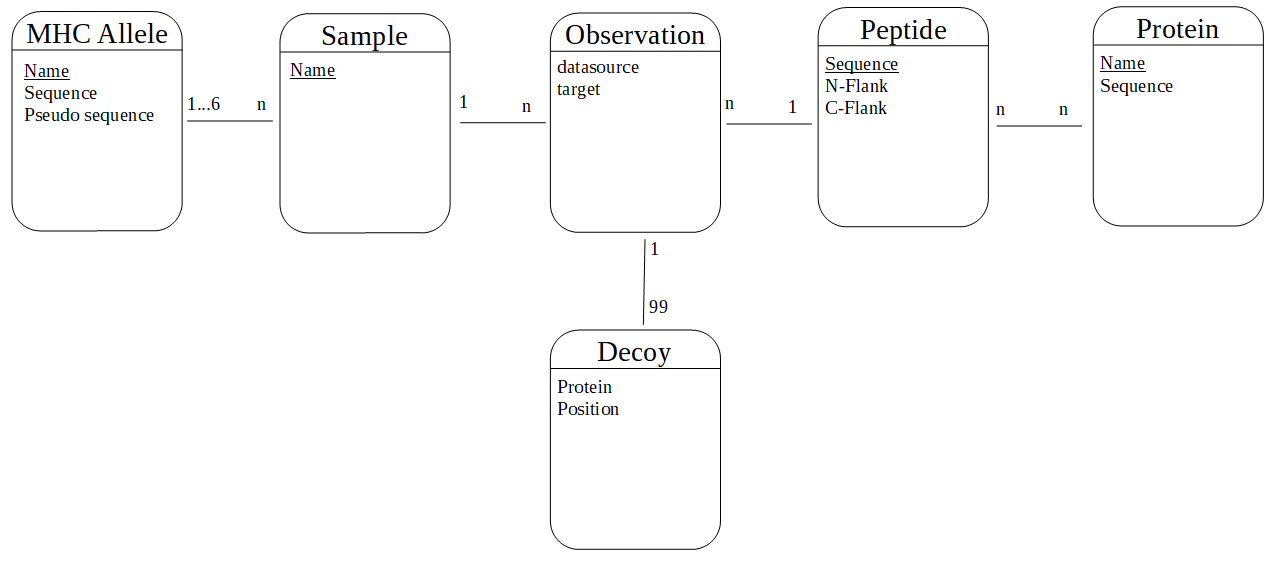
\includegraphics[width=1.0\textwidth]{class_diagram.png} 
			%	\caption{Illustration of data representation}
			%	\label{fig:data_rep}
			%\end{figure}
			
		Using the representation outlined above, we get the following Table \ref{tab:datasources} of observations, unique peptides and \gls{MHC} alleles occurring in our combined dataset.
		
	
		\begin{table}[H]
		\vskip 3mm
		\begin{center}
		\begin{small}
		\begin{sc}
		\begin{tabular}{| l | c | c c | c | c |}
		\hline
		Datasource			& samples		& \multicolumn{2}{c|}{observations} 	& unique  		& \gls{MHC} \\
						&			& \gls{SA}		& \gls{MA}		& peptides		& alleles \\
		\hline
		\hline
		University of Gdansk	& 271			& 293,334		& 1,256,916		& 390,959		& 104 \\
		Ligand Atlas			& 198			& 0			& 409,486		& 90,422		& 51 \\
		\hline
		Total				& 469			& 293,334		& 1,666,402		& 429,339		& 109 \\			
		\hline
		\end{tabular}
		\end{sc}
		\end{small}
		\caption{Overview of total dataset}
		\label{tab:datasources}
		\end{center}
		\vskip -7mm
		\end{table}
			
	
		\subsection{Decoy generation}
		\label{subsec:method_decoygeneration}
	
			Negative example (decoy) generation is very important, particularly due to the imbalanced nature of the dataset (see Subsection \ref{subsec:negative}). Our way of doing this is inspired by how the MHCflurry benchmark dataset was generated \cite{odonnell_mhcflurry_2020}. For each hit we sample 99 decoys. To match the observations' length distribution, the decoy peptides have the same length as their associated hits. To generate a decoy peptide we would randomly select any  protein from  the set of proteins observed in a sample. These are all proteins that any of the sample's peptides was mapped to. Then we randomly select a position within the protein as the start of the decoy peptide. This step should be improved in a next version of our model, as it might skew the decoys towards shorter proteins. Also, implicitly we (and other \gls{SOTA} models) assume that all proteins that a sample's peptides got mapped to must also be expressed in the sample. Based on this we take the absence of a peptide's observation as evidence for it actually not being presented. So, we assume that the data comes from high quality \gls{EL} experiments and that peptides are only matched to actually expressed proteins. We think that these assumptions need more scrutiny by the community and that  in a next step weighting examples by our confidence that they hold, might be beneficial.
			
			 The benchmark dataset of MHCflurry is used to test MHCflurry's performance. As seen in Subsection \ref{subsec:mhcflurry}, they generated 99 decoys from the same protein as the observation for the training of MHCflurry AP but only 2 decoys per observation for the training of MHCflurry PS. Ninety-nine decoys per hit fits better to the true distribution (see Subsection \ref{subsec:bg_biology_pathway}) but training on an imbalanced dataset might be an issue (see Subsection \ref{subsec:imbalanced}). Subsection \ref{subsec:netmhcpan} mentions that NetMHCpan 4.1 used roughly 18 decoys per hit. So, we consider using 19 or 99 decoys per hit in our hyper-parameter search (Section \ref{sec:hypsearch}). With regards to whether those should be chosen from the same protein as the observation or any protein observed within the sample, the implicit assumption for both is that absence of evidence is taken as evidence of absence. However, practically, there could be gene products that are too short to accommodate the 99 decoys per hit. So we decided to sample from all proteins observed during an experiment. 
		
		
		\subsection{Data splits}
		\label{subsec:split}
			Splitting the data into a train, test and validation set is not trivial, as: 
			\begin{itemize}
				\item[1.] We would like to assess generalization along 2 dimensions - primarily to unseen \gls{MHC} alleles and secondarily to unseen proteins
				\item[2.] Each observation can be associated with up to six \gls{MHC} alleles from which at least one is responsible for the presentation
				\item[3.] There are many homologues (see Subsection \ref{subsec:bg_biology_proteins}) in the human genome. Ideally, a group of homologues would not span different splits
			\end{itemize}
	
			\textbf{MHC allele dimension:} As each individual normally has at least one working copy of each \gls{HLA} gene (A/B/C), it is not possible to hold out a full gene. So, we hold out observations on the \gls{HLA} group level (e.g. HLA-A*01, ...). First we count how many observations belong to each \gls{HLA} group (from a donor/cell with at least one \gls{HLA} gene being in the group). The result can be found in Appendix Table \ref{tab:split_mhc}. We find that the groups are highly unequally represented in the dataset. To find at least 5 groups for each set, we perform the following steps until a satisfactory split is found. 
			
			First, we randomly assign \gls{HLA} groups (and the linked examples) to the validation set until its target number of examples is reached - overriding the standard training set assignment. Then we randomly assign allele groups to the test set until its target number of examples is reached - overriding any earlier assignment. If we assigned too few or too many we repeat. The final split can be found in Appendix Table \ref{tab:split_mhc}. Figure \ref{fig:mhc_split} illustrates this process which ensures that no validation or test \gls{MHC} group enters the training phase and no test \gls{MHC} group enters the validation or training phases.
			
			\begin{figure}
				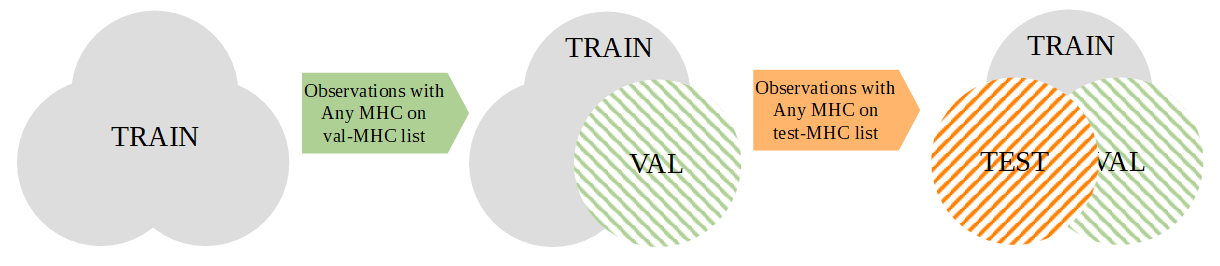
\includegraphics[width=1.0\textwidth]{split.png} 
				\caption{Illustration of splitting procedure}
				\label{fig:mhc_split}
			\end{figure}
	
			\textbf{Protein dimension:} Following this, we split off another validation and test set from the remaining training set. This second split is, however, based on an observation's mapped proteins not its linked \gls{MHC} alleles. Due to homology we cannot just split the dataset based on the protein names. There are many different approaches to deal with this. For example \cite{rao_evaluating_2019} have decided to go for sequence identity and ensure that no sequence in the test and train set have more than 25\% sequence identity. We feel that this approach might be the right one for the particular applications \cite{rao_evaluating_2019} had in mind - assessing for example overall protein structure. However, in our case we are more concerned with small local features - peptides. So we do not want to have any similarity of subsequences above 7 amino acids long. As checking this would be prohibitively computationally expensive, we chose another approach. We use the python networkx package, which allows to build and explore graph structures. With it we use the  Ensembl BioMart paralogue table \cite{ensembl_biomart_2021} to link related genes as well as proteins to their respective gene. We then randomly assign disconnected sub-graphs to the various splits until our target values are reached.
			
			Following the above, our dataset is split up into 5 sets. One training set, two validation sets and two test sets. Combining the two validation sets would be problematic. Let us assume an observation is part of the \gls{MHC} validation set. As the protein split is done on the remaining observations after the \gls{MHC} split, it cannot be part of the protein test or validation splits. However, it could still come from a protein, that is on the list of proteins defining the protein test set. Therefore, it is cleaner to keep these two perspectives independent.
			
			After the split, we obtain the partition of our data in Table \ref{tab:split}. Since generalization in the \gls{MHC} dimension is more important (as the peptides in our dataset already spread across the whole human genome), we assigned it a bigger proportion.
			
			\begin{table}[tb]
			\vskip 3mm
			\begin{center}
			\begin{small}
			\begin{sc}
			\begin{tabular}{| l | c | c c | c c |}
			\hline
			Split				& train			& val-prot			& test-prot			& val-mhc			& test-mhc \\
			\hline
			\hline
			% Total observations		& 1,407,876 (71.8\%) 	& 70,072 (3.6\%)		& 71,150 (3.6\%)		& 204,306 (10.4\%)	& 206,332 (10.5\%) \\
			% Single allele observations	& 205,591 (10.5\%)	& 10,149 (0.5\%)		& 11,056 (0.6\%)    	& 23,771 (1.2\%)  		& 42,767 (2.2\%) \\
			% Multiple allele observations& 1,202,285	(61.3\%)	& 59,923 (3.1\%)		& 60,094 (3.1\%)   		& 180,535 (9.2\%)		& 163,565 (8.3\%) \\		
			Total observations		& \makecell{1,408k \\ (71.8\%)}	 	& \makecell{70k \\ (3.6\%)}		& \makecell{71k \\ (3.6\%)}		& \makecell{204k \\ (10.4\%)}		& \makecell{206k \\ (10.5\%)} \\
			\hline
			Single allele			& \makecell{206k \\ (10.5\%)}		& \makecell{10k \\ (0.5\%)}		& \makecell{11k \\ (0.6\%)}    		& \makecell{24k \\ (1.2\%)}  		& \makecell{43k \\ (2.2\%)} \\
			\hline
			Multiple allele 		& \makecell{1,202k \\ (61.3\%)}		& \makecell{60k \\ (3.1\%)}		& \makecell{60k \\ (3.1\%)} 		& \makecell{181k \\ (9.2\%)}		& \makecell{164k \\ (8.3\%)} \\		

			\hline
			\end{tabular}
			\end{sc}
			\end{small}
			\caption{Observations per dataset split}
			\label{tab:split}
			\end{center}
			\vskip -7mm
			\end{table}	
	
	\section{Model Architecture} 
		One of the major \gls{ML} developments in the past few years has been transfer learning. This has been particularly successful in the domain of natural language processing where big networks like GPT-2 and T-5 have been trained on multiple GPUs for weeks and extensive text corpora and are now available in model zoos to download for everybody and fine-tune quickly to  their particular task. In this spirit, we adapt and use the pre-trained \gls{TAPE} transformer (see Subsection \ref{subsec:BERT}) as backbone for our model.
	
		\subsection{Tokenization and Embedding}
			The primary input into our model is the peptide's \gls{AA} sequence. If a peptide could be mapped to multiple proteins, then we check if all contexts are the same. If so, we provide the model with this context as input, otherwise not (as well as in the input to the decoy examples). The context consists of the up to 15 \glspl{AA} that occur to the 'left' of the peptide in its source protein's \gls{AA} sequence (the N-flank) as well as the up to 15 \glspl{AA} that occur to the 'right' of it (the C-flank). The 15 \glspl{AA} length was chosen to be compatible with MHCflurry and be able to use their benchmarking data. Finally, the model also receives the \gls{MHC} pseudo sequence as defined by NetMHCpan (see Subsection \ref{subsec:netmhcpan}) as  input.
			
			The input sequence starts with a $<$cls$>$ token. Then come the N-flank, peptide, C-flank and \gls{MHC} allele. In between those components and at the end of the sequence there are $<$sep$>$ tokens. The $<$sep$>$ are used in \gls{BERT} to separate sentences and the $<$cls$>$ is meant to be used for classification \cite{devlin_bert_2019}. 
			
			All of these components are represented by letters symbolizing amino acids. However, \gls{BERT} requires embedding vectors as input. At first a tokenizer splits the input sequence up into tokens and maps each to several integers - in our case token ID, position number and token type ID. Then, embedding layers assign a different learnt embedding vector to each token ID, position number and token type ID. The overall embedding is the sum of these vectors (in our case a 768 dimensional vector per token). Crucially, this embedding does not take into account its context. So every histidine at peptide position 3 will always result in the same embedding - independent of the other amino acids in the input sequence. In addition, there is an input mask with which it is possible to hide tokens from the model (set the mask to zero).
			
			To take advantage of the pretraining, we need to use the same token IDs as used by the \gls{TAPE} transformer. This represents each amino acid by a separate number. The tokenizer distinguishes 20 standard \glspl{AA}, the two non-standard \glspl{AA} (pyrrolysine, selenocystein) and unknown \glspl{AA} \cite{rao_evaluating_2019}. There exist alternative tokenizations. For example, several amino acids could be combined to form a single token.			
		
			Off the shelf, the \gls{TAPE} transformer supports only a single token type id. To make it easier for the model to distinguish between the various input parts, we use a novel representation of the input and extended the \gls{TAPE} model's token type embedding matrix to four different token types - one each for the N-flank, peptide, C-flank and \gls{MHC} protein. Their values are initialized with the \gls{TAPE} standard token type embedding values and will then diverge during training. 
			
			With regards to the position numbering, the N-flank begins with number one being the residue closest to the peptide (numbering from C- to N-terminus). This is done, so that the peptide's proximal amino acid is always at position 1 - even if the  N-flank is shorter than 15 \glspl{AA} long. In contrast, the peptide and C-flank position numbering is done from N- to C-terminus. For the \gls{MHC} pseudo sequence, we use the \gls{AA}'s position in the full \gls{MHC} amino acid sequence. This is done, so that in future, the model can be easily fine tuned to support full \gls{MHC} sequences. An example can be found in the Appendix.
		
		\subsection{Encoder}
			The resulting vectors from the embedding step are fed through the \gls{TAPE} encoder consisting of 12 self attention layers with 12 heads each. The output is again a vector of dimension 768 per position. This, however,  is now a contextual embedding for each position. This means,  that other elements of the input will have influenced this vector - so it will change if other positions in the input were to change.
			
		\subsection{Pooling}
		\label{subsec:pooling}
			The encoder produces as many vectors as input tokens. These cannot be fed directly into a \gls{MLP} which expects a fixed dimensional input. Pooling is necessary. \cite{toshniwal_cross-task_2020} showed that the optimal pooling operation is task dependent. BERTMHC (Subsection \ref{subsec:BERTMHC}) use average pooling. However, we felt that the meaning of the peptide, context and \gls{MHC} sequence are quite different and so we considered three options: to use averaging, to use an attention layer and to use the classification token's vector. We compare those as part of the hyper-parameter search (see Section \ref{sec:hypsearch}).
			
		\subsection{Head}
			The structure of our model's head is similar to the one used by BERTMHC \cite{cheng_bertmhc_2020}. It is also a \gls{MLP} consisting of two fully connected layers with a hidden dimension of 512. In contrast to BERTMHC we only have a single output neuron, with sigmoid activation. This is because we only estimate a presentation score and not binding affinity.
			
	\section{Training}
		The training procedure of our model is inspired by the  NNAlign\_MA framework and general results of \gls{MIL}. In the first training epoch we only use \gls{SA} data. Then follows a deconvolution phase. During this, we deconvolve each \gls{MA} observation by at first predicting the presentation score for each potentially responsible allele and then selecting the one with the highest score as the relevant allele. This means, that for forward-propagation and backward-propagation, the \gls{MA} example is treated as if coming from the relevant allele until the next deconvolution phase, which happens after each epoch. The relevant \gls{MHC} allele of the decoys, follows the one of the observation.
		
		For training we use standard binary cross entropy as loss function. The parameter gradients were calculated using standard back-propagation. We trained the full network (including encoder and embedding layers). The parameters were updated using the ADAM optimizer which adjusts each parameter's learning rate over time. We use its standard hyper-parameters from the original paper ($\beta_1 = 0.9, \beta_2 = 0.999$ \cite{kingma_adam_2017}). Although it is quite robust with regards to hyper-parameter choice, and adjusts the learning rates over time, a sensible choice of initial learning rate is still necessary \cite[page 306]{goodfellow_deep_2016}. We choose this as  part of the hyper-parameter search (see Section \ref{sec:hypsearch}). 
		
	\section{Evaluation}
		To shed light on what our model has learnt and to assess its quality, we performed:\\
		\textbf{- Evaluation} on the test sets\\
		\textbf{- Comparison} of our model to MHCflurry and NetMHCpan\\
		\textbf{- Model interpretation} by \gls{LIME} analysis of peptide, flanks and pseudo sequence feature importances, using motifs and by \gls{SHAP} analysis of peptide \glspl{AA} contributions
		
		\subsection{Evaluation on the test set}
		In Section \ref{sec:results_test_set} we evaluate our final model for \gls{AP}, \gls{ROC}-\gls{AUC} and accuracy (see Subsection \ref{subsec:imbalanced}) on the \gls{MHC} allele- and protein test sets (see Subsection \ref{subsec:split}).
		
		\subsection{Comparison to MHCflurry and NetMHCpan}
		\label{subsec:method_comparison}
		The MULTIALLELIC benchmark dataset of MHCflurry consists of 9,158,100 examples. Each has a peptide, N-flank (15 \gls{AA}), C-flank (15 \gls{AA}), up to six \gls{HLA} alleles as well as the predictions of NetMHCpan, MixMHCpred and MHCflurry for the example. \cite{odonnell_mhcflurry_2020} generated this dataset from 11 studies using \gls{EL} data. For each hit they randomly generated 99 decoys. A more detailed description and the full dataset is available in \cite[Supplement Data S1]{odonnell_mhcflurry_2020}. We run two evaluations on this - one on the whole dataset (9,158,100 examples) and one for which we removed examples of peptides that were already part of our training dataset (2,781,898 examples). For these we predict our model's presentation score, calculate performance metrics and plot \gls{PR} curves for MHCflurry, NetMHCpan and our model (ImmunoBERT).
		
		\subsection{Interpretation}
		\label{subsec:method_Interpretation}
			To reduce complexity, we restrict our interpretation of the model to 9-mer peptides and single-allele data. We used only the test set during interpretation. So, our model has not seen the data before. Therefore, the analysis demonstrates our model's ability to generalize to unseen \gls{MHC} proteins.

			\noindent \textbf{LIME analysis of all features:} We first assess the importance of all \gls{AA} features in the input-sequence. For this, we use the \gls{LIME} framework, as this is in general faster than \gls{SHAP} - in particular for many features (in our case ~73 amino acid positions). As described in Subsection \ref{subsec:interpretable_ai} we adapted the text version of \gls{LIME}. We implement the deactivation of a feature by setting the input mask token to zero. We use the standard cosine distance metric (in binary space) between the original example and the sampled examples. For each test set \gls{HLA} allele, we selected a random 500 observations and for each of those one decoy (total 1000 examples) to be explained. Each example gets explained by sampling a random 2000 feature combinations.

			For visualization, Figures \ref{fig:LIME_\HLAalleleI}, \ref{fig:LIME_\HLAalleleII} and \ref{fig:LIME_\HLAalleleIII} show in each bar the proportion of examples with a given importance-ranking. If for example the bright red bar (1st) of peptide position 9 showed 0.5, this means that 50\% of examples had this as the most important feature.
		
			\noindent \textbf{Sequence Motifs:} We want to utilize the very common sequence motif logos \cite{schneider_sequence_1990} to visualize for each test set \gls{HLA} allele, how often various amino acids occur at presented peptide positions. To do so, we generate 100,000 random 9-mer peptides from the human proteome (as well as their context). Then we predict for each of those 100,000 examples the presentation score for the \gls{HLA} protein concerned. We select the ones for which our model predicts presentation (presentation score $> 0.5$) and use them to create the allele dependent logo for our model (using the logomaker \cite{tareen_logomaker_2019} package). This analysis is similar to the one carried out by \cite{wu_deephlapan_2019}, which however use the 2\%  highest scoring peptides for the  model motif. Afterwards, we take the data from our test set and use all of the 9-mer peptides unambiguously presented by the \gls{HLA} allele to create another logo for the data as well.
			
			The created motif logos have the following form. For each of the nine peptide positions, a stack of \gls{AA} letters is displayed. The size of each letter is proportional to the \gls{AA}'s frequency at this position. Also, more frequent \glspl{AA} can be found on top. Each stack is then scaled with the position's \gls{IC}, resulting in a representation as bits \cite{schneider_sequence_1990}. The lower the position's entropy, the higher the \gls{IC} and, so, the logo. We do not display positions with \gls{IC} $< 0.5$ to avoid distraction. Amino acids with similar chemistry are coloured the same. 
			
			\noindent \textbf{SHAP analysis of peptide positions:} Finally, we look for additional insights by examining the average contribution of peptide amino acids using \gls{SHAP}. For each test set \gls{HLA} allele, we select a random five-hundred 9-mer single allele hits and one decoy per hit to explain from the test set. From these 1000 examples we also sample 250 as background distribution (see Subsection \ref{subsec:interpretable_ai}). The nine features in the peptide would result in a maximum of 512 feature subsets. We carry out the Kernel \gls{SHAP} analysis using a sample of 64 of these (see Subsection \ref{subsec:interpretable_ai}). For the whole process we ignore the flanks. In Figures \ref{fig:SHAP_\HLAalleleI}, \ref{fig:SHAP_\HLAalleleII} and \ref{fig:SHAP_\HLAalleleIII} we plot the average \gls{SHAP} value for each amino acid at each position.			


\chapter{Results}
\label{chapter:results}
	This chapter presents the results obtained by applying the methodologies from Chapter \ref{chapter:method}. First, we justify some of the parameters chosen before benchmarking our model to two alternative \gls{SOTA} models. Eventually, we use explainability techniques to analyse what our model has learnt about peptide presentation by three test set \gls{HLA} proteins.


	\section{Hyperparameter search and training}
	\label{sec:hypsearch}
		We searched parameters along 3 dimensions: pooling mechanism, decoys per hit and learning rate. We considered using the $<$cls$>$ tokens embedding, averaging and a classical attention mechanism (see Subsection \ref{subsec:pooling}) as pooling mechanism. Further, we compare using datasets enriched by 19 and 99 decoys per observation. Eventually, we try using 1e-04, 1e-05 and 1e-06 as initial learning rates. For the hyperparameter search, each model was trained on 10\% of the \gls{SA} data for 64,599 steps (one epoch for the 99 decoys per observation datasets and five epochs for the 19 decoys per observation datasets - so both of them have seen the same observations at least once).
		
		We evaluated each model on 10\% of the \gls{MHC}-validation and protein-validation set \footnote{our two validation sets, see Subsection \ref{subsec:split}} \gls{SA} data (using 99 decoys per hit). Table \ref{tab:hparam_e05} shows the result for the hyper-parameter search using a learning rate of 1e-05. The results for a learning rate of 1e-06 can be found in Appendix Table \ref{tab:hparam_e06} and show, that the learning happened too slow. Using a learning rate of 1e-04 would most of the time not result in any detected hits.
		
		Table \ref{tab:hparam_e05} shows various performance metrics (best column values in red) on our two validation sets for the 6 models described above at two points during their training. Different initializations might deliver different results, as mentioned above we didn't use the full dataset and the training will not have converged after 64,559 steps yet. However, given our limited computing resources and the time it takes to train transformers, we had to base our decision on these numbers.  Dependent on the chosen metric, one or the other pooling mechanism and one or the other hits-to-decoys ratio  looks best. In general, the unbalanced dataset (99 decoys per hit) at first (step 12,911) leads to quite poor classifiers in terms of \gls{ROC}-\gls{AUC} and \gls{AP}. However, after a full epoch they are able to make up most of this. In fact, as found by \cite{weiss_learning_2003}, models trained on an unbalanced dataset close to the actual data distribution (99 decoys per observation) show better accuracy. Actually, the models using only 19 decoys per observation have a worse accuracy than just always predicting negative. However, as we have seen in Subsection \ref{subsec:imbalanced} accuracy is not informative and reliable when dealing with highly imbalanced data \footnote{e.g. when the majority to minority class ratio is 999:1 a classifier always predicting the majority class  will have 99.9\% accuracy}. As we see in Table \ref{tab:hparam_e05} the models performing best on \gls{ROC}-\gls{AUC} and \gls{AP} all were trained using 19 decoys-per-hit. So we will use this. The table also  shows that using the classification token as input to the head had the best performance (in red) in 5 cases while the attention mechanism only had the best performance in 3 cases and the averaging in 2 cases. We will, therefore, train our final  model using the classification token's output as input to the model's head.
		
		\begin{table}[H]
			\vskip 3mm
			\begin{center}
			\begin{small}
			\begin{sc}
			\begin{tabular}{| c | c | c | c c c | c c c |}
			\hline
			\multirow{2}{*}{Pooling}		& \multirow{2}{*}{Decoys}		& after				& \multicolumn{3}{c|}{val-mhc}		& \multicolumn{3}{c|}{val-protein} \\
								&						& x steps				& {\tiny\makecell{\gls{ROC}\\ \gls{AUC}}}	& \gls{AP}		& Acc°  	& {\tiny\makecell{\gls{ROC}\\ \gls{AUC}}}	& \gls{AP}		& Acc° \\
			\hline
			\hline
			\multirow{4}{*}{Cls}		& \multirow{2}{*}{19}			& 12911				& 0.938 & 0.319 & 0.986 & 0.956 & 0.447 & 0.987 \\	
								& 						& 64559				& {\color{red}0.949} & 0.394 & 0.982 & {\color{red}0.964} & {\color{red}0.552} & 0.983 \\
								\cline{2-9}
								& \multirow{2}{*}{99}			& 12911				& 0.823 & 0.062 & 0.990 & 0.917 & 0.232 & 0.990 \\
								& 						& 64559				& 0.945 & 0.349 & {\color{red}0.991} & 0.960 & 0.492 & {\color{red}0.992} \\
			\cline{1-9}
			\multirow{4}{*}{Attn}		& \multirow{2}{*}{19}			& 12911				& 0.936 & 0.298 & 0.973 & 0.957 & 0.447 & 0.982 \\
								& 						& 64559				& 0.941 & {\color{red}0.410} & 0.983 & {\color{red}0.964} & 0.535 & 0.982 \\
								\cline{2-9}
								& \multirow{2}{*}{99}			& 12911				& 0.792 & 0.044 & 0.990 & 0.884 & 0.184 & 0.990 \\
								& 						& 64559				& 0.938 & 0.315 & 0.990 & 0.958 & 0.496 & {\color{red}0.992} \\
			\cline{1-9}
			\multirow{4}{*}{Avg}		& \multirow{2}{*}{19}			& 12911				& 0.926 & 0.252 & 0.982 & 0.954 & 0.417 & 0.985 \\
								& 						& 64559				& {\color{red}0.949} & 0.369 & 0.977 & 0.960 & 0.506 & 0.980 \\
								\cline{2-9}
								& \multirow{2}{*}{99}			& 12911				& 0.689 & 0.026 & 0.990 & 0.835 & 0.145 & 0.990 \\
								& 						& 64559				& 0.924 & 0.287 & 0.990 & 0.956 & 0.471 & {\color{red}0.992} \\
	
			\hline
			\end{tabular}
			\end{sc}
			\end{small}
			\caption{Performance comparison for a learning rate of 1e-05 (°... accuracy)}
			\label{tab:hparam_e05}
			\end{center}
			\vskip -7mm
		\end{table}	


		Table \ref{tab:training} shows how various metrics develop during its training. Due to time reasons and little improvement we stopped after epoch 5 and use this as our final model.
		
		\begin{table}[H]
			\vskip 3mm
			\begin{center}
			\begin{small}
			\begin{sc}
			\begin{tabular}{| c c | c c c | c c c |}	
			\hline
			\multicolumn{2}{|c|}{after}				& \multicolumn{3}{c|}{val-mhc}		& \multicolumn{3}{c|}{val-protein} \\
			epochs			& steps			& \gls{AP}	& {\tiny\makecell{\gls{ROC}\\ \gls{AUC}}}	& Acc°  	& \gls{AP} 	& {\tiny\makecell{\gls{ROC}\\\gls{AUC}}}	& Acc° \\
			\hline
			\hline
			1 & 128494 & 0.571 & 0.966 & 0.989 & 0.667 & 0.985 & 0.988 \\
			\hline
			2 & 1008417 & 0.646 & 0.976 & 0.992 & 0.762 & 0.993 & 0.993 \\
			\hline
			3 & 1888340 & 0.671 & 0.978 & 0.993 & 0.767 & 0.993 & 0.994 \\
			\hline
			4 & 2768263 & 0.673 & 0.978 & 0.992 & 0.768 & 0.993 & 0.993 \\
			\hline
			5 & 3648186 & 0.683 & 0.979 & 0.992 & 0.765 & 0.993 & 0.994 \\			
			\hline
			\end{tabular}
			\end{sc}
			\end{small}
			\caption{Performance comparison during training (°... accuracy)}
			\label{tab:training}
			\end{center}
			\vskip -7mm
		\end{table}	

	\section{Evaluation on the test set}
	\label{sec:results_test_set}

		To make sure we didn't overfit the hyperparameters to the validation set, Table \ref{tab:test} shows the test set performance of our selected final model. We see that the values are not very different from the ones for the validation set in Table \ref{tab:training}.

		\begin{table}[H]
			\vskip 3mm
			\begin{center}
			\begin{small}
			\begin{sc}
			\begin{tabular}{| c c | c c c | c c c |}	
			\hline
			\multicolumn{2}{|c|}{after}				& \multicolumn{3}{c|}{test-mhc}		& \multicolumn{3}{c|}{test-protein} \\
			epochs			& steps			& \gls{AP}		& {\tiny\makecell{\gls{ROC}\\ \gls{AUC}}}	& Acc°  	& \gls{AP} 	& {\tiny\makecell{\gls{ROC}\\ \gls{AUC}}}	&  Acc° \\
			\hline
			\hline
			\hline
			5 & 3648186 & 0.704 & 0.981 & 0.993 & 0.755 & 0.992 & 0.993 \\			
			\hline
			\end{tabular}
			\end{sc}
			\end{small}
			\caption{Performance on the test set (°... accuracy)}
			\label{tab:test}
			\end{center}
			\vskip -7mm
		\end{table}	

	
	\section{Benchmarking}
	\label{sec:results_benchmarking}
		Unluckily, there are no generally agreed upon standard benchmarking datasets available in our domain. However, \cite{odonnell_mhcflurry_2020} have curated a benchmark dataset (see Subsection \ref{subsec:method_comparison}). We ran the below analysis on the full dataset as well as on one in which we exclude peptides from our training set. We calculated the \gls{AP} as well as the \gls{ROC}-\gls{AUC} for MHCflurry, NetMHCpan and ImmunoBERT. For the full set we also plotted the \gls{PR}-curves for them (Table \ref{tab:benchmark_metrics}). The models were trained on different datasets. So any judgement about the advantageousness of the architectures is not valid. However, the comparison is useful to compare the practical predictive power of the models.

		For both datasets, our model shows an \gls{AP} in between MHCflurry and NetMHCpan. In particular, it does well for thresholds corresponding to intermediate recall levels. However, it achieves less \gls{ROC}-\gls{AUC} than the others, possibly caused by the sharp drop in performance for higher recall values. The performance on the reduced set is far worse for all models. So, also the other two models might have already seen similar peptides as were removed during their training. As we explicitly only removed ours, this skews the reduced dataset against our model.
		
		We decided to generate decoys once and show the model the same decoys in each epoch. This was done to ensure reproducibility of results. In contrast, NetMHCpan and MHCflurry resample decoys each epoch \cite{odonnell_mhcflurry_2020}. In hindsight, this might be a better design choice and might have led to later convergence during training of our model.

		\begin{table}[H]
			\vskip 3mm
			\begin{center}
			\begin{small}
			\begin{sc}
			\begin{tabular}{| c | l | c c | c | c c |}
			\hline
			& Model 	/ Metric			& \gls{AP}		& {\tiny\makecell{\gls{ROC}\\\gls{AUC}}} & \gls{PR}-Curve 	 \\
			\hline
			\hline
			\multirow{6}{*}{\rotatebox{90}{Full Dataset}}
			& NetMHCpan			& 0.327		& 0.916 & \multirow{3}{*}{\includegraphics[width=5.5cm]{PR.pdf} } 	\\	
			& MHCflurry				& 0.427		& 0.938 & 											\\	
			& ImmunoBERT			& 0.383		& 0.893 & 										\\
			& 					&			&	  & 											\\
			& 					&			&	  & 											\\
			& 					&			&	  & 											\\
			\hline
			\multirow{6}{*}{\rotatebox{90}{Reduced Dataset}}
			& NetMHCpan			& 0.151		& 0.873 & \multirow{3}{*}{\includegraphics[width=5.5cm]{PR_red.pdf} } \\	
			& MHCflurry				& 0.215		& 0.890 & 											\\	
			& ImmunoBERT			& 0.163		& 0.831 & 										\\
			& 					&			&	  & 											\\
			& 					&			&	  & 											\\
			& 					&			&	  & 											\\
			\hline
			\end{tabular}
			\end{sc}
			\end{small}
			\caption{Performance comparison on benchmark dataset}
			\label{tab:benchmark_metrics}
			\end{center}
			\vskip -7mm
		\end{table}	

		
			
	\section{Interpretation}
	\label{sec:results_interpretation}
		Next we use \gls{LIME}, motifs and \gls{SHAP} as described in Subsection \ref{subsec:method_Interpretation} to interpret our model's predictions for three selected test set \gls{HLA} proteins. We chose them to cover different \gls{HLA} genes and degrees of perceived matching between their data and model motifs. As there are too many test \gls{HLA} alleles to discuss within the boundaries of this thesis, we put the figures for the remaining test \gls{HLA} alleles into the Appendix. To improve readability all \gls{SHAP} values were multiplied by 100.

		\newpage	
		\subsection{\HLAalleleIname}
				\noindent \begin{figure}[H]
						\includegraphics[width=14.5cm]{lime_\HLAalleleI.pdf} 
						\captionof{figure}{\gls{LIME} feature importance rank distribution for \HLAalleleIname}
						\label{fig:LIME_\HLAalleleI}
				\end{figure} 

				\noindent \begin{minipage}[c][7cm][t]{8cm}
				\noindent Figure \ref{fig:LIME_\HLAalleleI} shows for each input position the proportion of examples in which this position had a certain importance ranking (see Subsection \ref{subsec:method_Interpretation}). The peptide's \glspl{AA} tend to be highly ranked. Its position 9 is ranked first in roughly half of the examples. The \gls{MHC} pseudo sequence positions display a high variance in their ranking distributions. Some positions tend to be particularly highly ranked - like 63, 73, 116 and 171. 
				\end{minipage}
				\begin{minipage}[r][7cm][t]{6cm}
					\includegraphics[width=5.7cm]{\HLAalleleI_actual.png}
					\includegraphics[width=5.7cm]{\HLAalleleI_\finalModel.png} 
					\vskip -1mm
					\captionof{figure}{Data(top) \& model motif}
					\label{fig:LOGO_\HLAalleleI}
				\end{minipage}

				\gls{MHC} positions 171 and 116 are located in the \gls{MHC}'s A and F pockets \cite{van_deutekom_zooming_2015} which both are supposed to house a peptide terminus \cite{stryhn_longer_2000}. This might explain what we see in the motifs of Figure \ref{fig:LOGO_\HLAalleleI} \footnote{motifs show the frequency of \glspl{AA} at positions in observed peptides (hits), Subsection \ref{subsec:method_Interpretation}}. A peptide C-terminus arginine (R) is very common and the N-terminus is enriched as well. In contrast, the significance of \gls{MHC} positions 73 (in pocket C) and 63 (in pocket B) is unclear. There might be confounding with other positions or some biological reason for this. For example pocket B could house peptide position 2 - also explaining the slightly elevated importance of this in Figure \ref{fig:LIME_\HLAalleleI}. This is just speculation and biological experiments are needed to confirm this.

				Finally, the flanks seem the least important in Figure \ref{fig:LIME_\HLAalleleI}. \cite{odonnell_mhcflurry_2020} also found that including them only results in a small but consistent improvement. Within the flanks, quite sensibly our model attributes most importance to peptide proximal positions.

				The data and model motifs in Figure \ref{fig:LOGO_\HLAalleleI} are not exactly the same. This might be because they were generated from different background distributions \footnote{While the data motif is based only on the peptides that were expressed in the samples of the test \gls{HLA} allele, the model motifs are based on the whole human genome - Subsection \ref{subsec:method_Interpretation}}. We argue below that also the \gls{SHAP} values are context, and so background distribution, dependent.

				\begin{figure}[H]
				\begin{subfigure}{.5\textwidth}
					\centering
					\includegraphics[width=6.5cm]{shap_\HLAalleleI_\finalModel_all.pdf}
				\end{subfigure}
				\begin{subfigure}{.5\textwidth}
					\centering
					\includegraphics[width=6.5cm]{shap_\HLAalleleI_\finalModel_scatter.pdf}
				\end{subfigure}
				\captionof{figure}{Mean \gls{SHAP} values (x 100) for \HLAalleleI examples}
				\label{fig:SHAP_\HLAalleleI}
				\end{figure}

				With regards to \gls{SHAP} values, Figure \ref{fig:SHAP_\HLAalleleI} left side shows the mean \gls{SHAP} value of each \gls{AA} at each peptide position \footnote{see Subsection \ref{subsec:method_Interpretation}}. We see the strong positive mean contribution of R at peptide position 9, making its high frequency in Figures \ref{fig:LOGO_\HLAalleleI} plausible. It also shows high values for V and T at position 2 which are also enriched in the model motif. \\

				\noindent \begin{minipage}[c][8.7cm][t]{9.3cm}
				 Intuitively, higher mean \gls{SHAP} values should be linked to more occurrences of the \gls{AA} at a position. Figure \ref{fig:SHAP_\HLAalleleI} right side depicts this relationship. For hits it seems to be positive - not so for decoys. To investigate this further, Figure \ref{fig:SHAP_\HLAalleleI_change} shows for each \gls{AA} the difference between its mean \gls{SHAP} value at position 8 in hits (dot) and in decoys (end of arrow). Especially the values for Asparagine N and Cysteine C change a lot. This demonstrates the context's importance for a feature's \gls{SHAP} value. So, high average \gls{SHAP} values need not lead to higher occurrences under all background distributions.

				
				\end{minipage}
				\begin{minipage}[r][8.7cm][t]{4.7cm}
					\centering
					\includegraphics[width=4.2cm]{shap_\HLAalleleI_\finalModel_change_8_mean.pdf}
					\captionof{figure}{position 8: change in \gls{SHAP} values}
					\label{fig:SHAP_\HLAalleleI_change}
				\end{minipage}
 

				%\begin{figure}
				%	\includegraphics[width=6cm]{shap_\HLAalleleI_\finalModel_change_1_mean.pdf}
				%	\captionof{figure}{Average 100xSHAP values}
				%	\label{fig:SHAP_\HLAalleleI_change_1_mean}
				%\end{figure}
			       

		\subsection{\HLAalleleIIname}
				\noindent \begin{figure}[H]
						\includegraphics[width=14.5cm]{lime_\HLAalleleII.pdf} 
						\captionof{figure}{\gls{LIME} feature importance rank distribution for \HLAalleleIIname}
						\label{fig:LIME_\HLAalleleII}
				\end{figure} 

				\noindent \begin{minipage}[c][14cm][t]{8cm}
				\noindent We see a similar picture in Figure \ref{fig:LIME_\HLAalleleII} as in Figure \ref{fig:LIME_\HLAalleleI}. The peptide is the most important element followed by the \gls{MHC} allele and the flanks are the least important. However, this time two positions in the peptide are of especially great importance - 2 and 9. This corresponds to what we see in the motifs in Figure \ref{fig:LOGO_\HLAalleleII} and in fact the \gls{SHAP} values in Figure \ref{fig:SHAP_\HLAalleleII}. 

				With regards to the \gls{MHC} protein, its most important position is 95. This is located in the F pocket \cite{van_deutekom_zooming_2015}. This makes sense given the high \gls{SHAP} values of peptide position 9. Its second most important position is 66 in pocket B. Given the enrichment of peptide position 2 by P and A we speculate that pocket B houses those. Indeed, \cite{liu_major_2011} claim that this is the case. Also the other \gls{MHC} alleles in our test set with a high specificity at peptide position 2 in the data motif (HLA-B*37:01, HLA-B*58:01 and HLA-B*58:02) show slightly elevated importances for pocket B positions (e.g. 66,  67) - see Appendix.

				\end{minipage}
				\begin{minipage}[r][14cm][t]{6cm}
					\includegraphics[width=6cm]{\HLAalleleII_actual.png}
					\includegraphics[width=6cm]{\HLAalleleII_\finalModel.png} 
					\captionof{figure}{Data (top) \& model motif}
					\label{fig:LOGO_\HLAalleleII}

					\includegraphics[width=6cm]{shap_\HLAalleleII_\finalModel_all.pdf}
					\captionof{figure}{Mean \gls{SHAP} values}
					\label{fig:SHAP_\HLAalleleII}
				\end{minipage}


		\subsection{\HLAalleleIIIname}
				\noindent \begin{figure}[H]
						\includegraphics[width=14.5cm]{lime_\HLAalleleIII.pdf} 
						\captionof{figure}{\gls{LIME} feature importance rank distribution for \HLAalleleIIIname}
						\label{fig:LIME_\HLAalleleIII}
				\end{figure} 

				\noindent \begin{minipage}[c][14cm][t]{8cm}
				\noindent Figure \ref{fig:LIME_\HLAalleleIII} shows a similar picture as Figures \ref{fig:LIME_\HLAalleleI} and \ref{fig:LIME_\HLAalleleII}. However, the data and model motifs in Figure \ref{fig:LOGO_\HLAalleleIII} are quite different. First, the model motif misses the enrichment  in particular by S and A at data motif position 8. Interestingly, those \glspl{AA} have relatively high mean \gls{SHAP} values in Figure \ref{fig:SHAP_\HLAalleleIII}. Also Figure \ref{fig:LIME_\HLAalleleIII} shows elevated importance of this position. So, this might just be caused by different background distributions between the sets used to generate the model (based on the whole human genome) and the data motif (based on test set examples). Next, the model motif shows an enrichment at position 4. This is primarily caused by E, which also has a high mean \gls{SHAP} value. Given the low \gls{IC} of this, the difference in motifs could be caused by chance. At peptide positions 2 and 3 the two motifs look very similar - except for ordering. With regards to \gls{MHC} positions 114 and 156 are especially important in Figure \ref{fig:LIME_\HLAalleleIII}. These lie close to each other in pocket E \cite{van_deutekom_zooming_2015} and might house one of the enriched peptide positions requiring further research.

				\end{minipage}
				\begin{minipage}[r][14cm][t]{6cm}
					\includegraphics[width=6cm]{\HLAalleleIII_actual.png}
					\includegraphics[width=6cm]{\HLAalleleIII_\finalModel.png} 
					\captionof{figure}{Data(top) \& model motif}
					\label{fig:LOGO_\HLAalleleIII}

					\includegraphics[width=6cm]{shap_\HLAalleleIII_\finalModel_all.pdf}
					\captionof{figure}{Mean \gls{SHAP} values}
					\label{fig:SHAP_\HLAalleleIII}
				\end{minipage}

				 


				%\begin{figure}
				%	\includegraphics[width=6cm]{shap_\HLAalleleI_\finalModel_change_1_mean.pdf}
				%	\captionof{figure}{Average 100xSHAP values}
				%	\label{fig:SHAP_\HLAalleleI_change_1_mean}
				%\end{figure}


\chapter{Conclusion and future work}
\label{chapter:conclusion}
	We have seen in Section \ref{sec:results_benchmarking} that our model based on the \gls{BERT} architecture was able to compete with current \gls{SOTA} models that have been developed over many years. This highlights \gls{BERT}'s high potential in this area. Then, we compared various pooling techniques and decoy to hit ratios in Section \ref{sec:hypsearch} and found that the best choice will depend on the evaluation metric. As a novel approach in Section \ref{sec:results_interpretation} we used the explainability techniques \gls{LIME} and \gls{SHAP} to find that our model learnt biologically sensible importance rankings and feature contributions. Namely, it placed particularly high importance on \glspl{AA} near the N- and C-termini of the peptide and varying \gls{MHC}  positions in the A, B and F pockets. In contrast, the flanks showed less importance, which explains why \cite{odonnell_mhcflurry_2020} found that including them only results in a small but consistent model improvement.  The motifs we found using our model followed broadly those observed in the data. As these analysis were all carried out on held out \gls{MHC} proteins, it also demonstrates the generalization ability of our model.

Given the high degree of imbalance in the data, we think that more advanced methods are required for decoy generation. Generative adversarial networks might be a way to achieve this. An alternative could also be to utilize the ability of transformer models to assess all positions of a whole sequence at once. As input the model would not only receive a single peptide but a longer sequence of amino acids. It could then be trained to identify the presented sub sequences. This would make the artificial generation of decoys and in particular the search for a good ratio between decoys and hits unnecessary.

	To summarize, this thesis has highlighted the high potential of transformer models for peptide presentation prediction and as a novelty applied advanced explanation techniques to this task, with which we could demonstrate biological relationships.
	
\chapter{Appendix}
	\vspace{-5mm}
	\section{MHC split}
		\vspace{-5mm}
		\begin{table}[H]
		\vskip 3mm
		\begin{center}
		\begin{footnotesize}
		\begin{sc}
		\begin{tabular}{| c c c | c c c | c c c |}
		\hline
		\multicolumn{3}{|c|}{HLA-A}					& \multicolumn{3}{|c|}{HLA-B}					&  \multicolumn{3}{|c|}{HLA-C} \\
		Group			& S°			& Hits	 		& Group		& S°			& Hits		 	& Group		& S°			& Hits \\
		\hline
		HLA-A01   		& 99			& 359,049		& HLA-B07   		& 66   			& 378,396		& HLA-C01 **	& 10   			&  36,665 \\
		HLA-A02   		& 156			& 505,417		& HLA-B08 * 		& 37   			& 128,339 		& HLA-C02   		& 73   			& 322,819\\
		HLA-A03   		& 92   			& 644,773		& HLA-B13   		& 18   			&  42,331 		& HLA-C03   		& 96   			& 392,462\\
		HLA-A11   		& 80   			& 200,286		& HLA-B14   		& 47   			& 219,850 		& HLA-C04   		& 114   		& 566,983\\
		HLA-A23   		& 25   			&  73,141		& HLA-B15   		& 75   			& 228,832 		& HLA-C05   		& 37   			& 416,633\\
		HLA-A24   		& 60   			& 299,863		& HLA-B18   		& 25   			& 177,056 		& HLA-C06   		& 75   			& 199,060\\
		HLA-A25   		&  3   			&  14,163		& HLA-B27   		& 54   			& 285,520 		& HLA-C07   		& 173   		& 614,980\\
		HLA-A26   		&  9   			&  16,779		& HLA-B35   		& 108   		& 572,469 		& HLA-C08   		& 48   			& 223,603\\
		HLA-A29   		& 24   			& 244,649		& HLA-B37 **	& 30   			&  74,723 		& HLA-C12   		&  9   			&  77,625\\
		HLA-A30   		& 16   			&  22,321		& HLA-B38   		&  5   			&  45,822 		& HLA-C14   		&  7   			&  34,824\\
		HLA-A31   		& 18   			& 199,800		& HLA-B39 *		&  6   			&  60,623 		& HLA-C15 **	&  5   			&  17,682\\
		HLA-A32   		& 39   			& 272,779		& HLA-B40   		& 43   			& 156,648 		& HLA-C16   		& 25   			&  58,074\\
		HLA-A33 ** 		&  2   			&   8,015		& HLA-B41   		&  2   			&  12,971 		& HLA-C17 **	&  4   			&  18,124\\
		HLA-A34 * 		&  2   			&   7,749		& HLA-B42 * 		&  1   			&   4,077 		& 			&			& \\
		HLA-A36 **   	&  1   			&   3,960		& HLA-B44   		& 83   			& 398,328 		& 			&			& \\
		HLA-A66 *  		&  1   			&   2,532		& HLA-B45   		& 17   			&  30,927 		& 			&			& \\
		HLA-A68   		& 75   			& 246,119		& HLA-B46 **	&  1   			&   1,203 		& 			& 			& \\
		HLA-A69   		& 22   			&  50,198		& HLA-B47 *		&  6   			&   3,720 		& 			&			& \\
		HLA-A74 **  		&  1   			&   3,543		& HLA-B49   		& 30   			&  78,815 		& 			&			& \\
					&			&			& HLA-B51 *		&  9   			&  29,332 		& 			&			& \\
					&			&			& HLA-B52 * 		&  1   			&   1,585 		& 			&			& \\
					&			&			& HLA-B53 * 		&  1   			&   2,883 		& 			&			& \\
					&			&			& HLA-B54 **	&  1   			&   1,622 		& 			&			& \\
					&			&			& HLA-B55   		&  7   			&  29,812 		& 			&			& \\
					&			&			& HLA-B56 * 		&  1   			&   1,780 		& 			&			& \\
					&			&			& HLA-B57   		&  8   			&  24,397 		& 			&			& \\
					&			&			& HLA-B58 **	& 24   			&  40,795 		& 			&			& \\
		\hline
		\end{tabular}
		\end{sc}
		\end{footnotesize}
		\caption{MHC groups in the datasets (°... samples, *... validation set, **... test set)}
		\label{tab:split_mhc}
		\end{center}
		\vskip -7mm
		\end{table}
			
	\section{Tokenization example}
	
		Peptide: 'LWDSAVSHF' \\
		N-flank: 'SVSHKFLSLPMLVRQ' \\
		C-flank: 'FSLPFKKSLLAALIL' \\
		MHC pseudo sequence: 'YYAGYREKYRQTDVNKLYLRYDSYTWAEWAYEWY' \\
		
		\noindent This will result in the following string: 
		\begin{center}
		`$<$cls$>$SVSHKFLSLPMLVRQ$<$sep$>$LWDSAVSHF$<$sep$>$FSLPFKKSLL\\AALIL$<$sep$>$YYAGYREKYRQTDVNKLYLRYDSYTWAEWAYEWY$<$sep$>$' 
		\end{center}
		
		\noindent This string will be tokenized into the following input token ids: 2, 22, 25, 22, 12, 14, 10, 15, 22, 15, 19, 16, 15, 25, 21, 20,  3, 15, 26,  8, 22,  5, 25, 22, 12, 10,  3, 10, 22, 15, 19, 10, 14, 14, 22, 15, 15,  5,  5, 15, 13, 15,  3, 28, 28,  5, 11, 28, 21,  9, 14, 28, 21, 20, 23,  8, 25, 17, 14, 15, 28, 15, 21, 28,  8, 22, 28, 23, 26,  5,  9, 26, 5, 28,  9, 26, 28,  3 \\
		
		\noindent These input token ids will be linked to the following token type ids: 2, 1, 1, 1, 1, 1, 1, 1, 1, 1, 1, 1, 1, 1, 1, 1, 1, 2, 2, 2, 2, 2, 2, 2, 2, 2, 2, 3, 3, 3, 3, 3, 3, 3, 3, 3, 3, 3, 3, 3, 3, 3, 3, 0, 0, 0, 0, 0, 0, 0, 0, 0, 0, 0, 0, 0, 0, 0, 0, 0, 0, 0, 0, 0, 0, 0, 0, 0, 0, 0, 0, 0, 0, 0, 0, 0, 0, 0 \\
		
		\noindent The corresponding position ids are: 0,  15,  14,  13,  12,  11,  10,   9,   8,   7,   6,   5,   4,   3,  2,   1,   0,   1,   2,   3,   4,   5,   6,   7,   8,   9,   0,   1,  2,   3,   4,   5,   6,   7,   8,   9,  10,  11,  12,  13,  14,  15,  0,   7,   9,  24,  45,  59,  62,  63,  66,  67,  69,  70,  73,  74,  76,  77,  80,  81,  84,  95,  97,  99, 114, 116, 118, 143, 147, 150,  152, 156, 158, 159, 163, 167, 171,   0 \\

		\noindent If all features should be considered, then every input mask position will be 1: 1, 1, 1, 1, 1, 1, 1, 1, 1, 1, 1, 1, 1, 1, 1, 1, 1, 1, 1, 1, 1, 1, 1, 1, 1, 1, 1, 1, 1, 1, 1, 1, 1, 1, 1, 1, 1, 1, 1, 1, 1, 1, 1, 1, 1, 1, 1, 1, 1, 1, 1, 1, 1, 1, 1, 1, 1, 1, 1, 1, 1, 1, 1, 1, 1, 1, 1, 1, 1, 1, 1, 1, 1, 1, 1, 1, 1, 1 \\


	\section{Hyperparameter search}
	
		\begin{table}[H]
			\vskip 3mm
			\begin{center}
			\begin{small}
			\begin{sc}
			\begin{tabular}{| c | c | c | c c c | c c c |}
			\hline
			\multirow{2}{*}{Pooling}		& \multirow{2}{*}{Decoys}		& after				& \multicolumn{3}{c|}{val-mhc}		& \multicolumn{3}{c|}{val-protein} \\
								&						& x steps				& {\tiny\makecell{ROC\\AUC}}	& \gls{AP}	& Acc°  	& {\tiny\makecell{ROC\\AUC}}	& \gls{AP}	& Acc° \\
			\hline
			\hline
			\multirow{4}{*}{Cls}		& \multirow{2}{*}{19}			& 12911				& 0.660 & 0.020 & 0.990 & 0.771 & 0.061 & 0.990 \\	
								& 						& 64559				& 0.902 & 0.209 & 0.974 & 0.943 & 0.356 & 0.975 \\
								\cline{2-9}
								& \multirow{2}{*}{99}			& 12911				& 0.584 & 0.013 & 0.990 & 0.689 & 0.033 & 0.990 \\
								& 						& 64559				& 0.721 & 0.027 & 0.990 & 0.835 & 0.119 & 0.990 \\
			\cline{1-9}
			\multirow{4}{*}{Attn}		& \multirow{2}{*}{19}			& 12911				& 0.649 & 0.018 & 0.990 & 0.774 & 0.073 & 0.990 \\
								& 						& 64559				& 0.902 & 0.210 & 0.975 & 0.937 & 0.349 & 0.975 \\
								\cline{2-9}
								& \multirow{2}{*}{99}			& 12911				& 0.594 & 0.014 & 0.990 & 0.694 & 0.034 & 0.990 \\
								& 						& 64559				& 0.731 & 0.029 & 0.990 & 0.829 & 0.132 & 0.990 \\
			\cline{1-9}
			\multirow{4}{*}{Avg}		& \multirow{2}{*}{19}			& 12911				& 0.657 & 0.020 & 0.990 & 0.776 & 0.081 & 0.990\\
								& 						& 64559				& 0.892 & 0.202 & 0.969 & 0.937 & 0.349 & 0.970 \\
								\cline{2-9}
								& \multirow{2}{*}{99}			& 12911				& 0.601 & 0.016 & 0.990 & 0.700 & 0.037 & 0.990 \\
								& 						& 64559				& 0.733 & 0.031 & 0.990 & 0.840 & 0.134 & 0.990 \\
	
			\hline
			\end{tabular}
			\end{sc}
			\end{small}
			\caption{Performance comparison for a learning rate of 1e-06 (°... accuracy)}
			\label{tab:hparam_e06}
			\end{center}
			\vskip -7mm
		\end{table}	

	\section{Interpretation}
		On the following pages, the charts for the remaining \gls{HLA} alleles that were note selected for detailed discussion in Section \ref{sec:results_interpretation} can be found. The methodology for constructing the charts was explained there  and in Subsection \ref{subsec:method_Interpretation}.

		\newpage
		\renewcommand{\HLAallele}{HLA-A3303}
		\renewcommand{\HLAalleleName}{HLA-A*33:03}
		\subsection{\HLAalleleName}
				\noindent \begin{minipage}[c][4.2cm][t]{7cm}
					\begin{center}
					\includegraphics[width=4cm]{\HLAallele_actual.png}
					\includegraphics[width=4cm]{\HLAallele_\finalModel.png} 
					\end{center}
				\end{minipage}
				\begin{minipage}[c][4.2cm][t]{7cm}
					\begin{center}
					\includegraphics[width=4.5cm]{shap_\HLAallele_\finalModel_all.pdf}
					\end{center}
				\end{minipage}
				
				\noindent \begin{figure}[H] {\centering
						\includegraphics[width=11cm]{lime_\HLAallele.pdf} 
						\captionof{figure}{Motifs (top left), mean \gls{SHAP} values (top right) and \gls{LIME} feature ranks}
						\label{fig:LIME_\HLAallele} }
				\end{figure}



		\renewcommand{\HLAallele}{HLA-A3601}
		\renewcommand{\HLAalleleName}{HLA-A*36:01}
		\subsection{\HLAalleleName}
				\noindent \begin{minipage}[c][4.2cm][t]{7cm}
					\begin{center}
					\includegraphics[width=4cm]{\HLAallele_actual.png}
					\includegraphics[width=4cm]{\HLAallele_\finalModel.png} 
					\end{center}
				\end{minipage}
				\begin{minipage}[c][4.2cm][t]{7cm}
					\begin{center}
					\includegraphics[width=4.5cm]{shap_\HLAallele_\finalModel_all.pdf}
					\end{center}
				\end{minipage}
				
				\noindent \begin{figure}[H] {\centering
						\includegraphics[width=11cm]{lime_\HLAallele.pdf} 
						\captionof{figure}{Motifs (top left), mean \gls{SHAP} values (top right) and \gls{LIME} feature ranks}
						\label{fig:LIME_\HLAallele} }
				\end{figure}

		\renewcommand{\HLAallele}{HLA-A7401}
		\renewcommand{\HLAalleleName}{HLA-A*74:01}
		\subsection{\HLAalleleName}
				\noindent \begin{minipage}[c][4.2cm][t]{7cm}
					\begin{center}
					\includegraphics[width=4cm]{\HLAallele_actual.png}
					\includegraphics[width=4cm]{\HLAallele_\finalModel.png} 
					\end{center}
				\end{minipage}
				\begin{minipage}[c][4.2cm][t]{7cm}
					\begin{center}
					\includegraphics[width=4.5cm]{shap_\HLAallele_\finalModel_all.pdf}
					\end{center}
				\end{minipage}
				
				\noindent \begin{figure}[H] {\centering
						\includegraphics[width=11cm]{lime_\HLAallele.pdf} 
						\captionof{figure}{Motifs (top left), mean \gls{SHAP} values (top right) and \gls{LIME} feature ranks}
						\label{fig:LIME_\HLAallele} }
				\end{figure}

		\renewcommand{\HLAallele}{HLA-B3701}
		\renewcommand{\HLAalleleName}{HLA-B*37:01}
		\subsection{\HLAalleleName}
				\noindent \begin{minipage}[c][4.2cm][t]{7cm}
					\begin{center}
					\includegraphics[width=4cm]{\HLAallele_actual.png}
					\includegraphics[width=4cm]{\HLAallele_\finalModel.png} 
					\end{center}
				\end{minipage}
				\begin{minipage}[c][4.2cm][t]{7cm}
					\begin{center}
					\includegraphics[width=4.5cm]{shap_\HLAallele_\finalModel_all.pdf}
					\end{center}
				\end{minipage}
				
				\noindent \begin{figure}[H] {\centering
						\includegraphics[width=11cm]{lime_\HLAallele.pdf} 
						\captionof{figure}{Motifs (top left), mean \gls{SHAP} values (top right) and \gls{LIME} feature ranks}
						\label{fig:LIME_\HLAallele} }
				\end{figure}

		\renewcommand{\HLAallele}{HLA-B4601}
		\renewcommand{\HLAalleleName}{HLA-B*46:01}
		\subsection{\HLAalleleName}
				\noindent \begin{minipage}[c][4.2cm][t]{7cm}
					\begin{center}
					\includegraphics[width=4cm]{\HLAallele_actual.png}
					\includegraphics[width=4cm]{\HLAallele_\finalModel.png} 
					\end{center}
				\end{minipage}
				\begin{minipage}[c][4.2cm][t]{7cm}
					\begin{center}
					\includegraphics[width=4.5cm]{shap_\HLAallele_\finalModel_all.pdf}
					\end{center}
				\end{minipage}
				
				\noindent \begin{figure}[H] {\centering
						\includegraphics[width=11cm]{lime_\HLAallele.pdf} 
						\captionof{figure}{Motifs (top left), mean \gls{SHAP} values (top right) and \gls{LIME} feature ranks}
						\label{fig:LIME_\HLAallele} }
				\end{figure}

		\renewcommand{\HLAallele}{HLA-B5801}
		\renewcommand{\HLAalleleName}{HLA-B*58:01}
		\subsection{\HLAalleleName}
				\noindent \begin{minipage}[c][4.2cm][t]{7cm}
					\begin{center}
					\includegraphics[width=4cm]{\HLAallele_actual.png}
					\includegraphics[width=4cm]{\HLAallele_\finalModel.png} 
					\end{center}
				\end{minipage}
				\begin{minipage}[c][4.2cm][t]{7cm}
					\begin{center}
					\includegraphics[width=4.5cm]{shap_\HLAallele_\finalModel_all.pdf}
					\end{center}
				\end{minipage}
				
				\noindent \begin{figure}[H] {\centering
						\includegraphics[width=11cm]{lime_\HLAallele.pdf} 
						\captionof{figure}{Motifs (top left), mean \gls{SHAP} values (top right) and \gls{LIME} feature ranks}
						\label{fig:LIME_\HLAallele} }
				\end{figure}

		\renewcommand{\HLAallele}{HLA-B5802}
		\renewcommand{\HLAalleleName}{HLA-B*58:02}
		\subsection{\HLAalleleName}
				\noindent \begin{minipage}[c][4.2cm][t]{7cm}
					\begin{center}
					\includegraphics[width=4cm]{\HLAallele_actual.png}
					\includegraphics[width=4cm]{\HLAallele_\finalModel.png} 
					\end{center}
				\end{minipage}
				\begin{minipage}[c][4.2cm][t]{7cm}
					\begin{center}
					\includegraphics[width=4.5cm]{shap_\HLAallele_\finalModel_all.pdf}
					\end{center}
				\end{minipage}
				
				\noindent \begin{figure}[H] {\centering
						\includegraphics[width=11cm]{lime_\HLAallele.pdf} 
						\captionof{figure}{Motifs (top left), mean \gls{SHAP} values (top right) and \gls{LIME} feature ranks}
						\label{fig:LIME_\HLAallele} }
				\end{figure}

		\renewcommand{\HLAallele}{HLA-C1502}
		\renewcommand{\HLAalleleName}{HLA-C*15:02}
		\subsection{\HLAalleleName}
				\noindent \begin{minipage}[c][4.2cm][t]{7cm}
					\begin{center}
					\includegraphics[width=4cm]{\HLAallele_actual.png}
					\includegraphics[width=4cm]{\HLAallele_\finalModel.png} 
					\end{center}
				\end{minipage}
				\begin{minipage}[c][4.2cm][t]{7cm}
					\begin{center}
					\includegraphics[width=4.5cm]{shap_\HLAallele_\finalModel_all.pdf}
					\end{center}
				\end{minipage}
				
				\noindent \begin{figure}[H] {\centering
						\includegraphics[width=11cm]{lime_\HLAallele.pdf} 
						\captionof{figure}{Motifs (top left), mean \gls{SHAP} values (top right) and \gls{LIME} feature ranks}
						\label{fig:LIME_\HLAallele} }
				\end{figure}

		\renewcommand{\HLAallele}{HLA-C1701}
		\renewcommand{\HLAalleleName}{HLA-C*17:01}
		\subsection{\HLAalleleName}
				\noindent \begin{minipage}[c][4.2cm][t]{7cm}
					\begin{center}
					\includegraphics[width=4cm]{\HLAallele_actual.png}
					\includegraphics[width=4cm]{\HLAallele_\finalModel.png} 
					\end{center}
				\end{minipage}
				\begin{minipage}[c][4.2cm][t]{7cm}
					\begin{center}
					\includegraphics[width=4.5cm]{shap_\HLAallele_\finalModel_all.pdf}
					\end{center}
				\end{minipage}
				
				\noindent \begin{figure}[H] {\centering
						\includegraphics[width=11cm]{lime_\HLAallele.pdf} 
						\captionof{figure}{Motifs (top left), mean \gls{SHAP} values (top right) and \gls{LIME} feature ranks}
						\label{fig:LIME_\HLAallele} }
				\end{figure}

\printglossaries

\printbibliography

%\bibliographystyle{plain}
%\bibliography{mybibfile}

%% You can include appendices like this:
% \appendix
% 
% \chapter{First appendix}
% 
% \section{First section}
% 
% Markers do not have to consider appendices. Make sure that your contributions
% are made clear in the main body of the dissertation (within the page limit).

\end{document}
